\documentclass[sigconf,nonacm,screen]{acmart}
\usepackage{filecontents}
\usepackage{textcomp}
\usepackage{pgfplots}
\usetikzlibrary{patterns}
\usepackage{ifthen}
\usepgfplotslibrary{groupplots}
\RequirePackage{keyval}
\usepackage{multirow}
\usepackage{multicol}
\usepackage{csvsimple}
\usepackage[utf8]{inputenc}
\newcounter{row}
\newcounter{col}
\usepackage{wrapfig}
\usepackage{textgreek}
\usepackage[inline]{enumitem}
\usetikzlibrary{matrix, positioning}
\usetikzlibrary{patterns,tikzmark}
\usetikzlibrary{matrix,decorations.pathreplacing,calc}
\usepackage{hf-tikz}
\usepackage{pifont}
\usepackage{subfig}
\usetikzlibrary{chains,fit,shapes}
\usetikzlibrary{arrows.meta,
    chains,
    positioning,
    shapes.symbols}
\usetikzlibrary{decorations,calligraphy}
\usepackage{pgfplotstable}
\usepgfplotslibrary{statistics}
%\pgfplotsset{compat=newest}
\usetikzlibrary{matrix,calc}
\usetikzlibrary{fit}
\usepackage{xfp}
\usepackage{mathtools}

\usetikzlibrary{positioning}

\usepackage{makecell}
%\usepackage{tabu}
\usepackage{tikz}
\usetikzlibrary{trees}

%\pgfplotsset{compat=1.8}
\pgfplotsset{compat=1.12}


\usepgfplotslibrary{fillbetween}

\usepackage{filecontents}
% \usetikzlibrary{pgfplots.groupplots}
% \pgfplotsset{compat=1.9}

% \usepackage[utf8]{inputenc}
% \usepackage[ngerman]{babel}
% \usepackage{pgfplots}
% \pgfplotsset{compat=1.9}
% \usetikzlibrary{
%   pgfplots.groupplots,
%   matrix
% }
% \usepackage{siunitx}

\newtheorem{theorem}{Theorem}
\newtheorem{definition}{Definition}
\newcommand{\eat}[1]{}

\definecolor{bluegreen}{RGB}{3, 166, 155}
\definecolor{pitchblack}{RGB}{0, 0, 0}
\definecolor{lightbeige}{RGB}{255, 251, 241}
\definecolor{mediumgray}{RGB}{183, 183, 183}
\definecolor{mygreen}{rgb}{0,0.6,0}
\definecolor{mygray}{rgb}{0.5,0.5,0.5}
\definecolor{mymauve}{rgb}{0.58,0,0.82}
\definecolor{keywords}{RGB}{255,0,90}
\definecolor{comments}{RGB}{0,0,113}
\definecolor{red}{RGB}{255,0,0}
\definecolor{green}{RGB}{0,255,0}
\definecolor{navy}{RGB}{0,0,128}
\definecolor{DarkGrenen}{RGB}{0,100,0}
\definecolor{DarkOliveGreen}{RGB}{85,107,47}
\definecolor{saddlebrown}{RGB}{139,69,19}
\definecolor{gold}{RGB}{252,194,1}
\definecolor{tug}{RGB}{247,1,70}
\definecolor{tugb}{RGB}{120,137,251}


\definecolor{blue0}{RGB}{153,153,153}
\definecolor{blue1}{RGB}{77,77,77}%
\definecolor{blue2}{RGB}{165,71,209}
\definecolor{blue3}{RGB}{77,10,142}
\definecolor{blue4}{RGB}{74,139,203}
\definecolor{blue5}{RGB}{40,40,190}

\definecolor{color1}{RGB}{100,149,237} % corn flower blue
\definecolor{color2}{RGB}{153,153,153} % light gray
\definecolor{color3}{RGB}{0,0,0} % black
\definecolor{color4}{RGB}{255,165,0} % orange
\definecolor{color5}{RGB}{255,69,0} % orange red
\definecolor{color6}{RGB}{77,77,77} % dark gray
\definecolor{color7}{RGB}{31,119,180}
\definecolor{color8}{RGB}{7,77,125}
\definecolor{color9}{RGB}{153,216,201}


\definecolor{teal1}{RGB}{31, 111, 111}
\definecolor{teal2}{RGB}{84, 161, 161}
\definecolor{teal3}{RGB}{159, 200, 200}

\definecolor{dred1}{RGB}{160, 0, 0}
\definecolor{dred2}{RGB}{196, 102, 102}
\definecolor{dred3}{RGB}{216, 166, 166}


\definecolor{dblue1}{RGB}{32, 102, 168}
\definecolor{dblue2}{RGB}{53, 148, 204}
\definecolor{dblue3}{RGB}{140, 197, 227}

\definecolor{totalcolor}{RGB}{2, 152, 215}
\definecolor{mvcolor}{RGB}{248, 163, 47}
\definecolor{dvcolor}{RGB}{203, 70, 39}



% Enable this two commands when you want to extract diagrams in extra files, then run "make"
\usetikzlibrary{external}
\tikzexternalize[prefix=plots/] %  activate

\usetikzlibrary{positioning}

\sloppy
\clubpenalty = 10000
\widowpenalty = 10000
\brokenpenalty = 10000
\frenchspacing


\makeatletter
\def\pgfplots@drawaxis@lines@preparediscont@for#1{%
        \ifnum\csname pgfplots@#1axisdiscontnum\endcsname>0
                \begingroup
                % this group employs several temporary dimension registers
                % and is therefor scoped:
                \let\disstart=\pgf@ya
                \let\disend=\pgf@yb
                \disend=\csname pgfplots@#1max@reg\endcsname
                \advance\disend by -\csname pgfplots@#1min@reg\endcsname
                \disend=\csname pgfplots@#1@veclength\endcsname\disend
                \ifcase\csname pgfplots@#1axisdiscontnum\endcsname\relax
                        % has already been checked above.
                \or
                        \def\discontstyle{decoration={zigzag,segment length=5pt, amplitude=2pt}}%
                        \advance \disend by -8pt
                \or
                        \def\discontstyle{decoration={ticks,segment length=4pt, amplitude=8pt}}%
                        \advance \disend by -4pt
                \fi
                \pgfplotscoordmath{#1}{datascaletrafo get params}%
                % if #1max + shift < 0pt  (shift is 0 without the scaling trafo)
                \ifdim\csname pgfplots@#1max@reg\endcsname<-\pgfplotsretvalb pt
                        % swap start and end
                        \disstart=\disend
                        \disend=2pt
                \else
                        \disstart=2pt
                \fi
                % carry local computations outside of group:
                \xdef\pgfplots@glob@TMPa{%
                        \noexpand\def\expandafter\noexpand\csname #1disstart\endcsname{\the\disstart}%
                        \noexpand\def\expandafter\noexpand\csname #1disend\endcsname{\the\disend}%
                        \noexpand\pgfkeysdef{/tikz/#1discont}{\noexpand\pgfkeysalso{\discontstyle}}%
                }%
                \endgroup
                \pgfplots@glob@TMPa
        \else
                \expandafter\def\csname #1disstart\endcsname{0pt}%
                \expandafter\def\csname #1disend\endcsname{0pt}%
                \pgfkeyslet{/tikz/#1discont}=\pgfutil@empty
        \fi
}%
\makeatother



\begin{document}
\title[Query Processing by Data Catalog]{Query Processing by Data Catalog}

\author{Saeed Fathollahzadeh} 
\orcid{0000-0003-3723-6191}
\affiliation{
\institution{Concordia University}
\country{Canada}}

\renewcommand{\shortauthors}{Saeed Fathollahzadeh}

\maketitle

    % %%%%%%%%%%%%%%%%%%%%%%%%%%%%%%%%%%%%%%%%%%%%%%%%%%%%%%%%%%%%%%%%%%%%%%%%%
%     \tikzsetnextfilename{Experiment1-Cost-EU-IT} 
%             \begin{figure}[!ht]
%                 \centering
%                 \makeatletter
\newcommand\resetstackedplots{
\makeatletter
\pgfplots@stacked@isfirstplottrue
\makeatother
\addplot [forget plot,draw=none] coordinates{(CatDB, 0) (CAAFERandomForest, 0) (CAAFETabPFN, 0)  (CatDBChain, 0)};
}
\makeatother

\begin{tikzpicture}

  \newcommand{\myaddplotcost}[7]{ 
    \addplot+[xshift=#4,fill=#3, draw=black,line width=0.3pt] 
    table[y=token_count_it1, col sep=comma, x=config, discard if singlconfig={No}{#2}{#1}{#5}{#6}]
    {../archive/VLDB2025/results/CostResults.csv};
    \label{#1_prompt}  

  };

  \newcommand{\myaddplotds}[6]{
    \resetstackedplots
    \myaddplotcost{CatDB}{#1}{dblue1}{#3}{#2}{0}{tug};
    \resetstackedplots
    \myaddplotcost{CAAFERandomForest}{#1}{color4}{#4}{#2}{0}{color4};
    \resetstackedplots
    \myaddplotcost{CAAFETabPFN}{#1}{black}{#5}{#2}{0}{black};
  };
\pgfplotsset{
    discard if singlconfig/.style n args={5}{
        x filter/.code={
            \edef\tempa{\thisrow{has_description}}
            \edef\tempb{#1}
            \ifx\tempa\tempb
              \edef\tempc{\thisrow{llm_model}}
                \edef\tempd{#2}
                  \ifx\tempc\tempd  
                  %
                    \edef\tempe{\thisrow{config}}
                    \edef\tempf{#3}
                    \ifx\tempe\tempf  
                    %
                      \edef\tempg{\thisrow{dataset_name_orig}}
                      \edef\temph{#4}
                      \ifx\tempg\temph
                      %
                        \edef\tempi{\thisrow{samples}}
                        \edef\tempj{#5}
                        \ifx\tempi\tempj                                      
                        \else
                        \def\pgfmathresult{inf}
                        \fi
                      %      
                      \else
                      \def\pgfmathresult{inf}
                      \fi
                  %           
                    \else
                    \def\pgfmathresult{inf}
                  \fi
                  %                
                  \else
                  \def\pgfmathresult{inf}
                  \fi
            \else
            \def\pgfmathresult{inf}
            \fi			
        }
    },
};   

\begin{axis}[
  ymin=0,
  ybar stacked,
  y tick label style={/pgf/number format/1000 sep={}},
  x tick label style={/pgf/number format/1000 sep={}},  
  scaled y ticks=false,
  axis line style={black, line width=0.3pt},
  enlarge y limits={0.09,upper},
  enlarge x limits=0.22,
  ylabel={Number of Tokens},
  xlabel={EU IT},
  log ticks with fixed point,
  xtick align=outside,
  xtick pos=left,
  ytick pos=left,
  yticklabel style = {font=\large},
  ylabel style = {font=\large, yshift=0pt, xshift=-3pt},
  xlabel style = {font=\large, yshift=5pt, xshift=-3pt},
  height=.5\columnwidth,
  width=.32\columnwidth,
  ymajorgrids=true,
  grid style=dotted,
  minor grid style={gray!70},
  %nodes near coords,
  %every node near coord/.append style={font=\fontsize{0.1pt}{0.1}, rotate=90, xshift=8pt, yshift=0pt},
  every axis plot/.append style={line width=0.4pt,mark options={scale=1.5,solid}},  
  xticklabel style = {font=\normalsize, xshift=0pt, yshift=3pt},
  legend image post style={line width=.5pt},          
  bar width=8pt,         
  ytick={0,1000,2000,3000},
  yticklabels={0, 1k, 2k, 3k},               
  every x tick/.style={ draw=none},
  xtick = data,
  symbolic x coords={CatDB, CAAFERandomForest, CAAFETabPFN, CatDBChain},
  xticklabels={},%{CatDB, CAAFE TabPFN, CAAFE R.Forest, CatDBChain},
  legend image code/.code={\draw [#1] (0cm,-0.1cm) rectangle (0.25cm,0.1cm); }, 
]
\myaddplotds{gemini-1.5-pro-latest}{EU-IT}{1pt}{4pt}{7pt}{9pt}
\end{axis}

\end{tikzpicture}
%                 \caption{Experiment1-Cost-EU-IT}
%             \end{figure} 
    
%     \tikzsetnextfilename{Experiment1-Cost-WiFi} 
%             \begin{figure}[!ht]
%                 \centering
%                 \makeatletter
\newcommand\resetstackedplots{
\makeatletter
\pgfplots@stacked@isfirstplottrue
\makeatother
\addplot [forget plot,draw=none] coordinates{(CatDB, 0) (CAAFERandomForest, 0) (CAAFETabPFN, 0)  (CatDBChain, 0)};
}
\makeatother

\begin{tikzpicture}

  \newcommand{\myaddplotcost}[7]{ 
    \addplot+[xshift=#4,fill=#3, draw=black,line width=0.3pt] 
    table[y=token_count_it1, col sep=comma, x=config, discard if singlconfig={No}{#2}{#1}{#5}{#6}]
    {../archive/VLDB2025/results/CostResults.csv};
    \label{#1_prompt}  

  };

  \newcommand{\myaddplotds}[6]{
    \resetstackedplots
    \myaddplotcost{CatDB}{#1}{dblue1}{#3}{#2}{0}{tug};
    \resetstackedplots
    \myaddplotcost{CAAFERandomForest}{#1}{color4}{#4}{#2}{0}{color4};
    \resetstackedplots
    \myaddplotcost{CAAFETabPFN}{#1}{black}{#5}{#2}{0}{black};
  };
\pgfplotsset{
    discard if singlconfig/.style n args={5}{
        x filter/.code={
            \edef\tempa{\thisrow{has_description}}
            \edef\tempb{#1}
            \ifx\tempa\tempb
              \edef\tempc{\thisrow{llm_model}}
                \edef\tempd{#2}
                  \ifx\tempc\tempd  
                  %
                    \edef\tempe{\thisrow{config}}
                    \edef\tempf{#3}
                    \ifx\tempe\tempf  
                    %
                      \edef\tempg{\thisrow{dataset_name_orig}}
                      \edef\temph{#4}
                      \ifx\tempg\temph
                      %
                        \edef\tempi{\thisrow{samples}}
                        \edef\tempj{#5}
                        \ifx\tempi\tempj                                      
                        \else
                        \def\pgfmathresult{inf}
                        \fi
                      %      
                      \else
                      \def\pgfmathresult{inf}
                      \fi
                  %           
                    \else
                    \def\pgfmathresult{inf}
                  \fi
                  %                
                  \else
                  \def\pgfmathresult{inf}
                  \fi
            \else
            \def\pgfmathresult{inf}
            \fi			
        }
    },
};   

\begin{axis}[
  ymin=0,
  ybar stacked,
  y tick label style={/pgf/number format/1000 sep={}},
  x tick label style={/pgf/number format/1000 sep={}},  
  scaled y ticks=false,
  axis line style={black, line width=0.3pt},
  enlarge y limits={0.09,upper},
  enlarge x limits=0.22,
  ylabel={},%{Number of Tokens},
  xlabel={Wifi},
  log ticks with fixed point,
  xtick align=outside,
  xtick pos=left,
  ytick pos=left,
  yticklabel style = {font=\large},
  ylabel style = {font=\large, yshift=0pt, xshift=-3pt},
  xlabel style = {font=\large, yshift=5pt, xshift=-3pt},
  height=.5\columnwidth,
  width=.32\columnwidth,
  ymajorgrids=true,
  grid style=dotted,
  minor grid style={gray!70},
  %nodes near coords,
  %every node near coord/.append style={font=\fontsize{0.1pt}{0.1}, rotate=90, xshift=8pt, yshift=0pt},
  every axis plot/.append style={line width=0.4pt,mark options={scale=1.5,solid}},  
  xticklabel style = {font=\normalsize, xshift=0pt, yshift=3pt},
  legend image post style={line width=.5pt},          
  bar width=8pt,         
  ytick={0,1000,2000},
  yticklabels={0, 1k, 2k},               
  every x tick/.style={ draw=none},
  xtick = data,
  symbolic x coords={CatDB, CAAFERandomForest, CAAFETabPFN, CatDBChain},
  xticklabels={},%{CatDB, CAAFE TabPFN, CAAFE R.Forest, CatDBChain},
  legend image code/.code={\draw [#1] (0cm,-0.1cm) rectangle (0.25cm,0.1cm); }, 
]
\myaddplotds{gemini-1.5-pro-latest}{WiFi}{1pt}{4pt}{7pt}{9pt}
\end{axis}

\end{tikzpicture}
%                 \caption{Experiment1-Cost-WiFi}
%             \end{figure}             
    
%     \tikzsetnextfilename{Experiment1-Cost-Etailing} 
%             \begin{figure}[!ht]
%                 \centering
%                 \makeatletter
\newcommand\resetstackedplots{
\makeatletter
\pgfplots@stacked@isfirstplottrue
\makeatother
\addplot [forget plot,draw=none] coordinates{(CatDB, 0) (CAAFERandomForest, 0) (CAAFETabPFN, 0)  (CatDBChain, 0)};
}
\makeatother

\begin{tikzpicture}

  \newcommand{\myaddplotcost}[7]{ 
    \addplot+[xshift=#4,fill=#3, draw=black,line width=0.3pt] 
    table[y=token_count_it1, col sep=comma, x=config, discard if singlconfig={No}{#2}{#1}{#5}{#6}]
    {../archive/VLDB2025/results/CostResults.csv};
    \label{#1_prompt}  

  };

  \newcommand{\myaddplotds}[6]{
    \resetstackedplots
    \myaddplotcost{CatDB}{#1}{dblue1}{#3}{#2}{0}{tug};
    \resetstackedplots
    \myaddplotcost{CAAFERandomForest}{#1}{color4}{#4}{#2}{0}{color4};
    \resetstackedplots
    \myaddplotcost{CAAFETabPFN}{#1}{black}{#5}{#2}{0}{black};
  };
\pgfplotsset{
    discard if singlconfig/.style n args={5}{
        x filter/.code={
            \edef\tempa{\thisrow{has_description}}
            \edef\tempb{#1}
            \ifx\tempa\tempb
              \edef\tempc{\thisrow{llm_model}}
                \edef\tempd{#2}
                  \ifx\tempc\tempd  
                  %
                    \edef\tempe{\thisrow{config}}
                    \edef\tempf{#3}
                    \ifx\tempe\tempf  
                    %
                      \edef\tempg{\thisrow{dataset_name_orig}}
                      \edef\temph{#4}
                      \ifx\tempg\temph
                      %
                        \edef\tempi{\thisrow{samples}}
                        \edef\tempj{#5}
                        \ifx\tempi\tempj                                      
                        \else
                        \def\pgfmathresult{inf}
                        \fi
                      %      
                      \else
                      \def\pgfmathresult{inf}
                      \fi
                  %           
                    \else
                    \def\pgfmathresult{inf}
                  \fi
                  %                
                  \else
                  \def\pgfmathresult{inf}
                  \fi
            \else
            \def\pgfmathresult{inf}
            \fi			
        }
    },
};   

\begin{axis}[
  ymin=0,
  ybar stacked,
  y tick label style={/pgf/number format/1000 sep={}},
  x tick label style={/pgf/number format/1000 sep={}},  
  scaled y ticks=false,
  axis line style={black, line width=0.3pt},
  enlarge y limits={0.09,upper},
  enlarge x limits=0.22,
  ylabel={},%{Number of Tokens},
  xlabel={Etailing},
  log ticks with fixed point,
  xtick align=outside,
  xtick pos=left,
  ytick pos=left,
  yticklabel style = {font=\large},
  ylabel style = {font=\large, yshift=0pt, xshift=-3pt},
  xlabel style = {font=\large, yshift=5pt, xshift=-3pt},
  height=.5\columnwidth,
  width=.32\columnwidth,
  ymajorgrids=true,
  grid style=dotted,
  minor grid style={gray!70},
  %nodes near coords,
  %every node near coord/.append style={font=\fontsize{0.1pt}{0.1}, rotate=90, xshift=8pt, yshift=0pt},
  every axis plot/.append style={line width=0.4pt,mark options={scale=1.5,solid}},  
  xticklabel style = {font=\normalsize, xshift=0pt, yshift=3pt},
  legend image post style={line width=.5pt},          
  bar width=8pt,         
  ytick={0,1000,2000,3000,4000,5000},
  yticklabels={0, 1k, 2k, 3k,4k,5k},               
  every x tick/.style={ draw=none},
  xtick = data,
  symbolic x coords={CatDB, CAAFERandomForest, CAAFETabPFN, CatDBChain},
  xticklabels={},%{CatDB, CAAFE TabPFN, CAAFE R.Forest, CatDBChain},
  legend image code/.code={\draw [#1] (0cm,-0.1cm) rectangle (0.25cm,0.1cm); }, 
]
\myaddplotds{gemini-1.5-pro-latest}{Etailing}{1pt}{4pt}{7pt}{9pt}
\end{axis}

\end{tikzpicture}
%                 \caption{Experiment1-Cost-Etailing}
%             \end{figure} 

%     \tikzsetnextfilename{Experiment1-Cost-Midwest-Survey} 
%             \begin{figure}[!ht]
%                 \centering
%                 \makeatletter
\newcommand\resetstackedplots{
\makeatletter
\pgfplots@stacked@isfirstplottrue
\makeatother
\addplot [forget plot,draw=none] coordinates{(CatDB, 0) (CAAFERandomForest, 0) (CAAFETabPFN, 0)  (CatDBChain, 0)};
}
\makeatother

\begin{tikzpicture}

  \newcommand{\myaddplotcost}[7]{ 
    \addplot+[xshift=#4,fill=#3, draw=black,line width=0.3pt] 
    table[y=token_count_it1, col sep=comma, x=config, discard if singlconfig={No}{#2}{#1}{#5}{#6}]
    {../archive/VLDB2025/results/CostResults.csv};
    \label{#1_prompt}  

  };

  \newcommand{\myaddplotds}[6]{
    \resetstackedplots
    \myaddplotcost{CatDB}{#1}{dblue1}{#3}{#2}{0}{tug};
    \resetstackedplots
    \myaddplotcost{CAAFERandomForest}{#1}{color4}{#4}{#2}{0}{color4};
    \resetstackedplots
    \myaddplotcost{CAAFETabPFN}{#1}{black}{#5}{#2}{0}{black};
  };
\pgfplotsset{
    discard if singlconfig/.style n args={5}{
        x filter/.code={
            \edef\tempa{\thisrow{has_description}}
            \edef\tempb{#1}
            \ifx\tempa\tempb
              \edef\tempc{\thisrow{llm_model}}
                \edef\tempd{#2}
                  \ifx\tempc\tempd  
                  %
                    \edef\tempe{\thisrow{config}}
                    \edef\tempf{#3}
                    \ifx\tempe\tempf  
                    %
                      \edef\tempg{\thisrow{dataset_name_orig}}
                      \edef\temph{#4}
                      \ifx\tempg\temph
                      %
                        \edef\tempi{\thisrow{samples}}
                        \edef\tempj{#5}
                        \ifx\tempi\tempj                                      
                        \else
                        \def\pgfmathresult{inf}
                        \fi
                      %      
                      \else
                      \def\pgfmathresult{inf}
                      \fi
                  %           
                    \else
                    \def\pgfmathresult{inf}
                  \fi
                  %                
                  \else
                  \def\pgfmathresult{inf}
                  \fi
            \else
            \def\pgfmathresult{inf}
            \fi			
        }
    },
};   

\begin{axis}[
  ymin=0,
  ybar stacked,
  y tick label style={/pgf/number format/1000 sep={}},
  x tick label style={/pgf/number format/1000 sep={}},  
  scaled y ticks=false,
  axis line style={black, line width=0.3pt},
  enlarge y limits={0.09,upper},
  enlarge x limits=0.22,
  ylabel={},%{Number of Tokens},
  xlabel={Survey},
  log ticks with fixed point,
  xtick align=outside,
  xtick pos=left,
  ytick pos=left,
  yticklabel style = {font=\large},
  ylabel style = {font=\large, yshift=0pt, xshift=-3pt},
  xlabel style = {font=\large, yshift=5pt, xshift=-3pt},
  height=.43\columnwidth,
  width=.32\columnwidth,
  ymajorgrids=true,
  grid style=dotted,
  minor grid style={gray!70},
  %nodes near coords,
  %every node near coord/.append style={font=\fontsize{0.1pt}{0.1}, rotate=90, xshift=8pt, yshift=0pt},
  every axis plot/.append style={line width=0.4pt,mark options={scale=1.5,solid}},  
  xticklabel style = {font=\normalsize, xshift=0pt, yshift=3pt},
  legend image post style={line width=.5pt},          
  bar width=8pt,         
  ytick={0,1000,2000,3000},
  yticklabels={0, 1k, 2k, 3k},               
  every x tick/.style={ draw=none},
  xtick = data,
  symbolic x coords={CatDB, CAAFERandomForest, CAAFETabPFN, CatDBChain},
  xticklabels={},%{CatDB, CAAFE TabPFN, CAAFE R.Forest, CatDBChain},
  legend image code/.code={\draw [#1] (0cm,-0.1cm) rectangle (0.25cm,0.1cm); }, 
]
\myaddplotds{gemini-1.5-pro-latest}{Midwest-Survey}{1pt}{4pt}{7pt}{9pt}
\end{axis}

\end{tikzpicture}
%                 \caption{Experiment1-Cost-Midwest-Survey}
%             \end{figure} 

%     \tikzsetnextfilename{Experiment1-Cost-Utility} 
%             \begin{figure}[!ht]
%                 \centering
%                 \makeatletter
\newcommand\resetstackedplots{
\makeatletter
\pgfplots@stacked@isfirstplottrue
\makeatother
\addplot [forget plot,draw=none] coordinates{(CatDB, 0) (CAAFERandomForest, 0) (CAAFETabPFN, 0)  (CatDBChain, 0)};
}
\makeatother

\begin{tikzpicture}

  \newcommand{\myaddplotcost}[7]{ 
    \addplot+[xshift=#4,fill=#3, draw=black,line width=0.3pt] 
    table[y=token_count_it1, col sep=comma, x=config, discard if singlconfig={No}{#2}{#1}{#5}{#6}]
    {../archive/VLDB2025/results/CostResults.csv};
    \label{#1_prompt}  

  };

  \newcommand{\myaddplotds}[6]{
    \resetstackedplots
    \myaddplotcost{CatDB}{#1}{dblue1}{#3}{#2}{0}{tug};
    \resetstackedplots
    \myaddplotcost{CAAFERandomForest}{#1}{color4}{#4}{#2}{0}{color4};
    \resetstackedplots
    \myaddplotcost{CAAFETabPFN}{#1}{black}{#5}{#2}{0}{black};
  };
\pgfplotsset{
    discard if singlconfig/.style n args={5}{
        x filter/.code={
            \edef\tempa{\thisrow{has_description}}
            \edef\tempb{#1}
            \ifx\tempa\tempb
              \edef\tempc{\thisrow{llm_model}}
                \edef\tempd{#2}
                  \ifx\tempc\tempd  
                  %
                    \edef\tempe{\thisrow{config}}
                    \edef\tempf{#3}
                    \ifx\tempe\tempf  
                    %
                      \edef\tempg{\thisrow{dataset_name_orig}}
                      \edef\temph{#4}
                      \ifx\tempg\temph
                      %
                        \edef\tempi{\thisrow{samples}}
                        \edef\tempj{#5}
                        \ifx\tempi\tempj                                      
                        \else
                        \def\pgfmathresult{inf}
                        \fi
                      %      
                      \else
                      \def\pgfmathresult{inf}
                      \fi
                  %           
                    \else
                    \def\pgfmathresult{inf}
                  \fi
                  %                
                  \else
                  \def\pgfmathresult{inf}
                  \fi
            \else
            \def\pgfmathresult{inf}
            \fi			
        }
    },
};   

\begin{axis}[
  ymin=0,
  ybar stacked,
  y tick label style={/pgf/number format/1000 sep={}},
  x tick label style={/pgf/number format/1000 sep={}},  
  scaled y ticks=false,
  axis line style={black, line width=0.3pt},
  enlarge y limits={0.09,upper},
  enlarge x limits=0.22,
  ylabel={},%{Number of Tokens},
  xlabel={Utility},
  log ticks with fixed point,
  xtick align=outside,
  xtick pos=left,
  ytick pos=left,
  yticklabel style = {font=\large},
  ylabel style = {font=\large, yshift=0pt, xshift=-3pt},
  xlabel style = {font=\large, yshift=5pt, xshift=-3pt},
  height=.43\columnwidth,
  width=.3\columnwidth,
  ymajorgrids=true,
  grid style=dotted,
  minor grid style={gray!70},
  %nodes near coords,
  %every node near coord/.append style={font=\fontsize{0.1pt}{0.1}, rotate=90, xshift=8pt, yshift=0pt},
  every axis plot/.append style={line width=0.4pt,mark options={scale=1.5,solid}},  
  xticklabel style = {font=\normalsize, xshift=0pt, yshift=3pt},
  legend image post style={line width=.5pt},          
  bar width=12pt,         
  ytick={0,1000,2000,3000},
  yticklabels={0, 1k, 2k,3k},               
  every x tick/.style={ draw=none},
  xtick = data,
  symbolic x coords={CatDB, CAAFERandomForest, CAAFETabPFN, CatDBChain},
  xticklabels={},%{CatDB, CAAFE TabPFN, CAAFE R.Forest, CatDBChain},
  legend image code/.code={\draw [#1] (0cm,-0.1cm) rectangle (0.25cm,0.1cm); }, 
]
\myaddplotds{gemini-1.5-pro-latest}{Utility}{9pt}{4pt}{7pt}{9pt}
\end{axis}

\end{tikzpicture}
%                 \caption{Experiment1-Cost-Utility}
%             \end{figure} 

% \tikzsetnextfilename{Experiment1-Cost-Yelp} 
%             \begin{figure}[!ht]
%                 \centering
%                 \makeatletter
\newcommand\resetstackedplots{
\makeatletter
\pgfplots@stacked@isfirstplottrue
\makeatother
\addplot [forget plot,draw=none] coordinates{(CatDBChain, 0) (CAAFERandomForest, 0) (CAAFETabPFN, 0)  (CatDB, 0)};
}
\makeatother

\begin{tikzpicture}

  \newcommand{\myaddplotcost}[7]{ 
    \addplot+[xshift=#4,fill=#3, draw=black,line width=0.3pt] 
    table[y=token_count_it1, col sep=comma, x=config, discard if singlconfig={No}{#2}{#1}{#5}{#6}]
    {../archive/VLDB2025/results/CostResults.csv};
    \label{#1_prompt}  

  };

  \newcommand{\myaddplotcostchain}[7]{ 
    \addplot+[xshift=#4,fill=#3, draw=black,line width=0.3pt] 
    table[y=token_count_it1, col sep=comma, x=config, discard if singlconfig={No}{#2}{#1}{#5}{#6}]
    {../archive/VLDB2025/results/CostResults.csv};
    \label{#1_prompt}  
     
    \addplot+[xshift=#4,fill=#3, draw=black,line width=0.3pt] 
    table[y=pp_token_count_it1, col sep=comma, x=config, discard if singlconfig={No}{#2}{#1}{#5}{#6}]
    {../archive/VLDB2025/results/CostResults.csv};
    \label{#1_pp_prompt}  
      
    \addplot+[xshift=#4,fill=#3, draw=black,line width=0.3pt] 
    table[y=pp_token_count_err_it1, col sep=comma, x=config, discard if singlconfig={No}{#2}{#1}{#5}{#6}]
    {../archive/VLDB2025/results/CostResults.csv};
    \label{#1_pp_err}  

    \addplot+[xshift=#4,fill=#3, draw=black,line width=0.3pt] 
    table[y=fe_token_count_it1, col sep=comma, x=config, discard if singlconfig={No}{#2}{#1}{#5}{#6}]
    {../archive/VLDB2025/results/CostResults.csv};
    \label{#1_fe_prompt}         
  };

  \newcommand{\myaddplotds}[6]{
    \resetstackedplots
    \myaddplotcostchain{CatDBChain}{#1}{tug}{#3}{#2}{0}{tug};
    \resetstackedplots
    \myaddplotcost{CAAFERandomForest}{#1}{color4}{#4}{#2}{0}{color4};
    \resetstackedplots
    \myaddplotcost{CAAFETabPFN}{#1}{black}{#5}{#2}{0}{black};
  };
\pgfplotsset{
    discard if singlconfig/.style n args={5}{
        x filter/.code={
            \edef\tempa{\thisrow{has_description}}
            \edef\tempb{#1}
            \ifx\tempa\tempb
              \edef\tempc{\thisrow{llm_model}}
                \edef\tempd{#2}
                  \ifx\tempc\tempd  
                  %
                    \edef\tempe{\thisrow{config}}
                    \edef\tempf{#3}
                    \ifx\tempe\tempf  
                    %
                      \edef\tempg{\thisrow{dataset_name_orig}}
                      \edef\temph{#4}
                      \ifx\tempg\temph
                      %
                        \edef\tempi{\thisrow{samples}}
                        \edef\tempj{#5}
                        \ifx\tempi\tempj                                      
                        \else
                        \def\pgfmathresult{inf}
                        \fi
                      %      
                      \else
                      \def\pgfmathresult{inf}
                      \fi
                  %           
                    \else
                    \def\pgfmathresult{inf}
                  \fi
                  %                
                  \else
                  \def\pgfmathresult{inf}
                  \fi
            \else
            \def\pgfmathresult{inf}
            \fi			
        }
    },
};   

\begin{axis}[
  ymin=0,
  ybar stacked,
  y tick label style={/pgf/number format/1000 sep={}},
  x tick label style={/pgf/number format/1000 sep={}},  
  scaled y ticks=false,
  axis line style={black, line width=0.3pt},
  enlarge y limits={0.09,upper},
  enlarge x limits=0.22,
  ylabel={},%{Number of Tokens},
  xlabel={Yelp},
  log ticks with fixed point,
  xtick align=outside,
  xtick pos=left,
  ytick pos=left,
  yticklabel style = {font=\large},
  ylabel style = {font=\large, yshift=0pt, xshift=-3pt},
  xlabel style = {font=\large, yshift=5pt, xshift=-3pt},
  height=.43\columnwidth,
  width=.32\columnwidth,
  ymajorgrids=true,
  grid style=dotted,
  minor grid style={gray!70},
  %nodes near coords,
  %every node near coord/.append style={font=\fontsize{0.1pt}{0.1}, rotate=90, xshift=8pt, yshift=0pt},
  every axis plot/.append style={line width=0.4pt,mark options={scale=1.5,solid}},  
  xticklabel style = {font=\normalsize, xshift=0pt, yshift=3pt},
  legend image post style={line width=.5pt},          
  bar width=12pt,         
  ytick={0,5000, 10000,15000, 20000,25000},
  yticklabels={0, 5k, 10k, 15k, 20k, 25k},               
  every x tick/.style={ draw=none},
  xtick = data,
  symbolic x coords={CatDBChain, CAAFERandomForest, CAAFETabPFN, CatDB},
  xticklabels={},%{CatDB, CAAFE TabPFN, CAAFE R.Forest, CatDBChain},
  legend image code/.code={\draw [#1] (0cm,-0.1cm) rectangle (0.25cm,0.1cm); }, 
]
\myaddplotds{gemini-1.5-pro-latest}{Yelp}{4pt}{12pt}{7pt}{9pt}
\end{axis}

\end{tikzpicture}
%                 \caption{Experiment1-Cost-Yelp}
%             \end{figure}             
            
    % \tikzsetnextfilename{Experiment1-Cost-10-Credit-g} 
    %         \begin{figure}[!ht]
    %             \centering
    %             \makeatletter
\newcommand\resetstackedplots{
\makeatletter
\pgfplots@stacked@isfirstplottrue
\makeatother
\addplot [forget plot,draw=none] coordinates{(gemini-1.5-pro-latest, 0) (llama3-70b-8192, 0) (gpt-4o, 0)};
}
\makeatother

\begin{tikzpicture}

  \newcommand{\myaddplotcost}[7]{ 
    \addplot+[xshift=#4,fill=#3, draw=black,line width=0.3pt] 
    table[y=tokens_count, col sep=comma, x=llm_model, discard if singlconfig={No}{#2}{#1}{#5}{#6}]
    {../archive/SIGMOD2025-Results/CostResults.csv};
    \label{#1_prompt}  

  };

  \newcommand{\myaddplotds}[6]{
    \resetstackedplots
    \myaddplotcost{CatDBChain}{#1}{tug}{#3}{#2}{0}{dred1};
    \resetstackedplots
    \myaddplotcost{CatDB}{#1}{dblue1}{#4}{#2}{0}{tug};
    \resetstackedplots
    \myaddplotcost{CAAFERandomForest}{#1}{color4}{#5}{#2}{0}{color4};
    \resetstackedplots
    \myaddplotcost{CAAFETabPFN}{#1}{black}{#6}{#2}{0}{black};
  };
\pgfplotsset{
    discard if singlconfig/.style n args={5}{
        x filter/.code={
            \edef\tempa{\thisrow{has_description}}
            \edef\tempb{#1}
            \ifx\tempa\tempb
              \edef\tempc{\thisrow{llm_model}}
                \edef\tempd{#2}
                  \ifx\tempc\tempd  
                  %
                    \edef\tempe{\thisrow{config}}
                    \edef\tempf{#3}
                    \ifx\tempe\tempf  
                    %
                      \edef\tempg{\thisrow{dataset_name_orig}}
                      \edef\temph{#4}
                      \ifx\tempg\temph
                      %
                        \edef\tempi{\thisrow{samples}}
                        \edef\tempj{#5}
                        \ifx\tempi\tempj                                      
                        \else
                        \def\pgfmathresult{inf}
                        \fi
                      %      
                      \else
                      \def\pgfmathresult{inf}
                      \fi
                  %           
                    \else
                    \def\pgfmathresult{inf}
                  \fi
                  %                
                  \else
                  \def\pgfmathresult{inf}
                  \fi
            \else
            \def\pgfmathresult{inf}
            \fi			
        }
    },
};   

\begin{axis}[
  ymin=0,
  ybar stacked,
  y tick label style={/pgf/number format/1000 sep={}},
  x tick label style={/pgf/number format/1000 sep={}},  
  scaled y ticks=false,
  axis line style={black, line width=0.3pt},
  enlarge y limits={0.09,upper},
  enlarge x limits=0.07,
  ylabel={Number of Tokens},
  xlabel={},
  log ticks with fixed point,
  xtick align=outside,
  xtick pos=left,
  ytick pos=left,
  yticklabel style = {font=\large},
  ylabel style = {font=\large, yshift=0pt, xshift=-3pt},
  height=.53\columnwidth,
  width=.66\columnwidth,
  ymajorgrids=true,
  grid style=dotted,
  minor grid style={gray!70},
  %nodes near coords,
  %every node near coord/.append style={font=\fontsize{0.1pt}{0.1}, rotate=90, xshift=8pt, yshift=0pt},
  every axis plot/.append style={line width=0.4pt,mark options={scale=1.5,solid}},  
  xticklabel style = {font=\normalsize, xshift=0pt, yshift=3pt},
  legend image post style={line width=.5pt},          
  bar width=8pt,         
  ytick={0,10000,20000,30000,40000},
  yticklabels={0, 10k, 20k, 30k,40k},               
  every x tick/.style={ draw=none},
  xtick = data,
  symbolic x coords={gemini-1.5-pro-latest, llama3-70b-8192, gpt-4o},
  xticklabels={\hspace{0.3cm}Gemini-1.5, \hspace{0.1cm}Llama3-70b, \hspace{-0.64cm}GPT-4o},
  legend image code/.code={\draw [#1] (0cm,-0.1cm) rectangle (0.25cm,0.1cm); }, 
]
\myaddplotds{gemini-1.5-pro-latest}{Credit-g}{0pt}{8pt}{16pt}{24pt}
\myaddplotds{llama3-70b-8192}{Credit-g}{-11pt}{-3pt}{5pt}{13pt}
\myaddplotds{gpt-4o}{Credit-g}{-22pt}{-14pt}{-6pt}{2pt}
\end{axis}

\end{tikzpicture}
    %             \caption{Experiment1-Cost-10-Credit-g}
    %         \end{figure} 

    % \tikzsetnextfilename{Experiment1-Cost-10-Diabetes} 
    %         \begin{figure}[!ht]
    %             \centering
    %             \makeatletter
\newcommand\resetstackedplots{
\makeatletter
\pgfplots@stacked@isfirstplottrue
\makeatother
\addplot [forget plot,draw=none] coordinates{(gemini-1.5-pro-latest, 0) (llama3-70b-8192, 0) (gpt-4o, 0)};
}
\makeatother

\begin{tikzpicture}

  \newcommand{\myaddplotcost}[7]{ 
    \addplot+[xshift=#4,fill=#3, draw=black,line width=0.3pt] 
    table[y=tokens_count, col sep=comma, x=llm_model, discard if singlconfig={No}{#2}{#1}{#5}{#6}]
    {../archive/SIGMOD2025-Results/CostResults.csv};
    \label{#1_prompt}  

  };

  \newcommand{\myaddplotds}[6]{
    \resetstackedplots
   \myaddplotcost{CatDB}{#1}{dblue1}{#3}{#2}{0}{tug};
    \resetstackedplots    
    \myaddplotcost{CatDBChain}{#1}{tug}{#4}{#2}{0}{dred1};
    \resetstackedplots
    \myaddplotcost{CAAFERandomForest}{#1}{color4}{#5}{#2}{0}{color4};
    \resetstackedplots
    \myaddplotcost{CAAFETabPFN}{#1}{black}{#6}{#2}{0}{black};
  };
\pgfplotsset{
    discard if singlconfig/.style n args={5}{
        x filter/.code={
            \edef\tempa{\thisrow{has_description}}
            \edef\tempb{#1}
            \ifx\tempa\tempb
              \edef\tempc{\thisrow{llm_model}}
                \edef\tempd{#2}
                  \ifx\tempc\tempd  
                  %
                    \edef\tempe{\thisrow{config}}
                    \edef\tempf{#3}
                    \ifx\tempe\tempf  
                    %
                      \edef\tempg{\thisrow{dataset_name_orig}}
                      \edef\temph{#4}
                      \ifx\tempg\temph
                      %
                        \edef\tempi{\thisrow{samples}}
                        \edef\tempj{#5}
                        \ifx\tempi\tempj                                      
                        \else
                        \def\pgfmathresult{inf}
                        \fi
                      %      
                      \else
                      \def\pgfmathresult{inf}
                      \fi
                  %           
                    \else
                    \def\pgfmathresult{inf}
                  \fi
                  %                
                  \else
                  \def\pgfmathresult{inf}
                  \fi
            \else
            \def\pgfmathresult{inf}
            \fi			
        }
    },
};   

\begin{axis}[
  ymin=0,
  ybar stacked,
  y tick label style={/pgf/number format/1000 sep={}},
  x tick label style={/pgf/number format/1000 sep={}},  
  scaled y ticks=false,
  axis line style={black, line width=0.3pt},
  enlarge y limits={0.09,upper},
  enlarge x limits=0.07,
  ylabel={Number of Tokens},
  xlabel={},
  log ticks with fixed point,
  xtick align=outside,
  xtick pos=left,
  ytick pos=left,
  yticklabel style = {font=\large},
  ylabel style = {font=\large, yshift=0pt, xshift=-3pt},
  height=.53\columnwidth,
  width=.66\columnwidth,
  ymajorgrids=true,
  grid style=dotted,
  minor grid style={gray!70},
  %nodes near coords,
  %every node near coord/.append style={font=\fontsize{0.1pt}{0.1}, rotate=90, xshift=8pt, yshift=0pt},
  every axis plot/.append style={line width=0.4pt,mark options={scale=1.5,solid}},  
  xticklabel style = {font=\normalsize, xshift=0pt, yshift=3pt},
  legend image post style={line width=.5pt},          
  bar width=8pt,         
  ytick={0,10000,20000,30000,40000},
  yticklabels={0, 10k, 20k, 30k,40k},               
  every x tick/.style={ draw=none},
  xtick = data,
  symbolic x coords={gemini-1.5-pro-latest, llama3-70b-8192, gpt-4o},
  xticklabels={\hspace{0.3cm}Gemini-1.5, \hspace{0.1cm}Llama3-70b, \hspace{-0.64cm}GPT-4o},
  legend image code/.code={\draw [#1] (0cm,-0.1cm) rectangle (0.25cm,0.1cm); }, 
]
\myaddplotds{gemini-1.5-pro-latest}{Diabetes}{0pt}{8pt}{16pt}{24pt}
\myaddplotds{llama3-70b-8192}{Diabetes}{-11pt}{-3pt}{5pt}{13pt}
\myaddplotds{gpt-4o}{Diabetes}{-22pt}{-14pt}{-6pt}{2pt}
\end{axis}

\end{tikzpicture}
    %             \caption{Experiment1-Cost-10-Diabetes}
    %         \end{figure} 

    % \tikzsetnextfilename{Experiment1-Cost-10-Nomao} 
    % \begin{figure}[!ht]
    %     \centering
    %     \makeatletter
\newcommand\resetstackedplots{
\makeatletter
\pgfplots@stacked@isfirstplottrue
\makeatother
\addplot [forget plot,draw=none] coordinates{(gemini-1.5-pro-latest, 0) (llama3-70b-8192, 0) (gpt-4o, 0)};
}
\makeatother

\begin{tikzpicture}

  \newcommand{\myaddplotcost}[7]{ 
    \addplot+[xshift=#4,fill=#3, draw=black,line width=0.3pt] 
    table[y=tokens_count, col sep=comma, x=llm_model, discard if singlconfig={No}{#2}{#1}{#5}{#6}]
    {../archive/SIGMOD2025-Results/CostResults.csv};
    \label{#1_prompt}  

  };

  \newcommand{\myaddplotds}[6]{
    \resetstackedplots
    \myaddplotcost{CatDBChain}{#1}{tug}{#3}{#2}{0}{dred1};
    \resetstackedplots
    \myaddplotcost{CatDB}{#1}{dblue1}{#4}{#2}{0}{tug};
    \resetstackedplots
    \myaddplotcost{CAAFERandomForest}{#1}{color4}{#5}{#2}{0}{color4};
    \resetstackedplots
    \myaddplotcost{CAAFETabPFN}{#1}{black}{#6}{#2}{0}{black};
  };
\pgfplotsset{
    discard if singlconfig/.style n args={5}{
        x filter/.code={
            \edef\tempa{\thisrow{has_description}}
            \edef\tempb{#1}
            \ifx\tempa\tempb
              \edef\tempc{\thisrow{llm_model}}
                \edef\tempd{#2}
                  \ifx\tempc\tempd  
                  %
                    \edef\tempe{\thisrow{config}}
                    \edef\tempf{#3}
                    \ifx\tempe\tempf  
                    %
                      \edef\tempg{\thisrow{dataset_name_orig}}
                      \edef\temph{#4}
                      \ifx\tempg\temph
                      %
                        \edef\tempi{\thisrow{samples}}
                        \edef\tempj{#5}
                        \ifx\tempi\tempj                                      
                        \else
                        \def\pgfmathresult{inf}
                        \fi
                      %      
                      \else
                      \def\pgfmathresult{inf}
                      \fi
                  %           
                    \else
                    \def\pgfmathresult{inf}
                  \fi
                  %                
                  \else
                  \def\pgfmathresult{inf}
                  \fi
            \else
            \def\pgfmathresult{inf}
            \fi			
        }
    },
};   

\begin{axis}[
  ymin=0,
  ybar stacked,
  y tick label style={/pgf/number format/1000 sep={}},
  x tick label style={/pgf/number format/1000 sep={}},  
  scaled y ticks=false,
  axis line style={black, line width=0.3pt},
  enlarge y limits={0.09,upper},
  enlarge x limits=0.07,
  ylabel={Number of Tokens},
  xlabel={},
  log ticks with fixed point,
  xtick align=outside,
  xtick pos=left,
  ytick pos=left,
  yticklabel style = {font=\large},
  ylabel style = {font=\large, yshift=0pt, xshift=-3pt},
  height=.53\columnwidth,
  width=.66\columnwidth,
  ymajorgrids=true,
  grid style=dotted,
  minor grid style={gray!70},
  %nodes near coords,
  %every node near coord/.append style={font=\fontsize{0.1pt}{0.1}, rotate=90, xshift=8pt, yshift=0pt},
  every axis plot/.append style={line width=0.4pt,mark options={scale=1.5,solid}},  
  xticklabel style = {font=\normalsize, xshift=0pt, yshift=3pt},
  legend image post style={line width=.5pt},          
  bar width=8pt,         
  ytick={0,50000,100000,150000,200000},
  yticklabels={0, 50k, 100k, 150k,200k},               
  every x tick/.style={ draw=none},
  xtick = data,
  symbolic x coords={gemini-1.5-pro-latest, llama3-70b-8192, gpt-4o},
  xticklabels={\hspace{0.3cm}Gemini-1.5, \hspace{0.1cm}Llama3-70b, \hspace{-0.64cm}GPT-4o},
  legend image code/.code={\draw [#1] (0cm,-0.1cm) rectangle (0.25cm,0.1cm); }, 
]
\myaddplotds{gemini-1.5-pro-latest}{Nomao}{0pt}{8pt}{16pt}{24pt}
\myaddplotds{llama3-70b-8192}{Nomao}{-11pt}{-3pt}{5pt}{13pt}
\myaddplotds{gpt-4o}{Nomao}{-22pt}{-14pt}{-6pt}{2pt}
\end{axis}

\end{tikzpicture}
    %     \caption{Experiment1-Cost-10-Nomao}
    % \end{figure} 

    % \tikzsetnextfilename{Experiment1-Cost-10-Gas-Drift} 
    % \begin{figure}[!ht]
    %     \centering
    %     \makeatletter
\newcommand\resetstackedplots{
\makeatletter
\pgfplots@stacked@isfirstplottrue
\makeatother
\addplot [forget plot,draw=none] coordinates{(gemini-1.5-pro-latest, 0) (llama3-70b-8192, 0) (gpt-4o, 0)};
}
\makeatother

\begin{tikzpicture}

  \newcommand{\myaddplotcost}[7]{ 
    \addplot+[xshift=#4,fill=#3, draw=black,line width=0.3pt] 
    table[y=tokens_count, col sep=comma, x=llm_model, discard if singlconfig={No}{#2}{#1}{#5}{#6}]
    {../archive/SIGMOD2025-Results/CostResults.csv};
    \label{#1_prompt}  

  };

  \newcommand{\myaddplotds}[6]{
    \resetstackedplots
    \myaddplotcost{CatDBChain}{#1}{tug}{#3}{#2}{0}{dred1};
    \resetstackedplots
    \myaddplotcost{CatDB}{#1}{dblue1}{#4}{#2}{0}{tug};
    \resetstackedplots
    \myaddplotcost{CAAFERandomForest}{#1}{color4}{#5}{#2}{0}{color4};
    \resetstackedplots
    \myaddplotcost{CAAFETabPFN}{#1}{black}{#6}{#2}{0}{black};
  };
\pgfplotsset{
    discard if singlconfig/.style n args={5}{
        x filter/.code={
            \edef\tempa{\thisrow{has_description}}
            \edef\tempb{#1}
            \ifx\tempa\tempb
              \edef\tempc{\thisrow{llm_model}}
                \edef\tempd{#2}
                  \ifx\tempc\tempd  
                  %
                    \edef\tempe{\thisrow{config}}
                    \edef\tempf{#3}
                    \ifx\tempe\tempf  
                    %
                      \edef\tempg{\thisrow{dataset_name_orig}}
                      \edef\temph{#4}
                      \ifx\tempg\temph
                      %
                        \edef\tempi{\thisrow{samples}}
                        \edef\tempj{#5}
                        \ifx\tempi\tempj                                      
                        \else
                        \def\pgfmathresult{inf}
                        \fi
                      %      
                      \else
                      \def\pgfmathresult{inf}
                      \fi
                  %           
                    \else
                    \def\pgfmathresult{inf}
                  \fi
                  %                
                  \else
                  \def\pgfmathresult{inf}
                  \fi
            \else
            \def\pgfmathresult{inf}
            \fi			
        }
    },
};   

\begin{axis}[
  ymin=0,
  ybar stacked,
  y tick label style={/pgf/number format/1000 sep={}},
  x tick label style={/pgf/number format/1000 sep={}},  
  scaled y ticks=false,
  axis line style={black, line width=0.3pt},
  enlarge y limits={0.09,upper},
  enlarge x limits=0.07,
  ylabel={Number of Tokens},
  xlabel={},
  log ticks with fixed point,
  xtick align=outside,
  xtick pos=left,
  ytick pos=left,
  yticklabel style = {font=\large},
  ylabel style = {font=\large, yshift=0pt, xshift=-3pt},
  height=.53\columnwidth,
  width=.66\columnwidth,
  ymajorgrids=true,
  grid style=dotted,
  minor grid style={gray!70},
  %nodes near coords,
  %every node near coord/.append style={font=\fontsize{0.1pt}{0.1}, rotate=90, xshift=8pt, yshift=0pt},
  every axis plot/.append style={line width=0.4pt,mark options={scale=1.5,solid}},  
  xticklabel style = {font=\normalsize, xshift=0pt, yshift=3pt},
  legend image post style={line width=.5pt},          
  bar width=8pt,         
  ytick={0,10000,20000,30000,40000},
  yticklabels={0, 10k, 20k, 30k,40k},               
  every x tick/.style={ draw=none},
  xtick = data,
  symbolic x coords={gemini-1.5-pro-latest, llama3-70b-8192, gpt-4o},
  xticklabels={\hspace{0.3cm}Gemini-1.5, \hspace{0.1cm}Llama3-70b, \hspace{-0.64cm}GPT-4o},
  legend image code/.code={\draw [#1] (0cm,-0.1cm) rectangle (0.25cm,0.1cm); }, 
]
\myaddplotds{gemini-1.5-pro-latest}{Gas-Drift}{0pt}{8pt}{16pt}{24pt}
\myaddplotds{llama3-70b-8192}{Gas-Drift}{-11pt}{-3pt}{5pt}{13pt}
\myaddplotds{gpt-4o}{Gas-Drift}{-22pt}{-14pt}{-6pt}{2pt}
\end{axis}

\end{tikzpicture}
    %     \caption{Experiment1-Cost-10-Gas-Drift}
    % \end{figure} 

    % \tikzsetnextfilename{Experiment1-Cost-10-Volkert} 
    % \begin{figure}[!ht]
    %     \centering
    %     \makeatletter
\newcommand\resetstackedplots{
\makeatletter
\pgfplots@stacked@isfirstplottrue
\makeatother
\addplot [forget plot,draw=none] coordinates{(gemini-1.5-pro-latest, 0) (llama3-70b-8192, 0) (gpt-4o, 0)};
}
\makeatother

\begin{tikzpicture}

  \newcommand{\myaddplotcost}[7]{ 
    \addplot+[xshift=#4,fill=#3, draw=black,line width=0.3pt] 
    table[y=tokens_count, col sep=comma, x=llm_model, discard if singlconfig={No}{#2}{#1}{#5}{#6}]
    {../archive/SIGMOD2025-Results/CostResults.csv};
    \label{#1_prompt}  

  };

  \newcommand{\myaddplotds}[6]{
    \resetstackedplots
    \myaddplotcost{CatDBChain}{#1}{tug}{#3}{#2}{0}{dred1};
    \resetstackedplots
    \myaddplotcost{CatDB}{#1}{dblue1}{#4}{#2}{0}{tug};
    \resetstackedplots
    \myaddplotcost{CAAFERandomForest}{#1}{color4}{#5}{#2}{0}{color4};
    \resetstackedplots
    \myaddplotcost{CAAFETabPFN}{#1}{black}{#6}{#2}{0}{black};
  };
\pgfplotsset{
    discard if singlconfig/.style n args={5}{
        x filter/.code={
            \edef\tempa{\thisrow{has_description}}
            \edef\tempb{#1}
            \ifx\tempa\tempb
              \edef\tempc{\thisrow{llm_model}}
                \edef\tempd{#2}
                  \ifx\tempc\tempd  
                  %
                    \edef\tempe{\thisrow{config}}
                    \edef\tempf{#3}
                    \ifx\tempe\tempf  
                    %
                      \edef\tempg{\thisrow{dataset_name_orig}}
                      \edef\temph{#4}
                      \ifx\tempg\temph
                      %
                        \edef\tempi{\thisrow{samples}}
                        \edef\tempj{#5}
                        \ifx\tempi\tempj                                      
                        \else
                        \def\pgfmathresult{inf}
                        \fi
                      %      
                      \else
                      \def\pgfmathresult{inf}
                      \fi
                  %           
                    \else
                    \def\pgfmathresult{inf}
                  \fi
                  %                
                  \else
                  \def\pgfmathresult{inf}
                  \fi
            \else
            \def\pgfmathresult{inf}
            \fi			
        }
    },
};   

\begin{axis}[
  ymin=0,
  ybar stacked,
  y tick label style={/pgf/number format/1000 sep={}},
  x tick label style={/pgf/number format/1000 sep={}},  
  scaled y ticks=false,
  axis line style={black, line width=0.3pt},
  enlarge y limits={0.09,upper},
  enlarge x limits=0.07,
  ylabel={Number of Tokens},
  xlabel={},
  log ticks with fixed point,
  xtick align=outside,
  xtick pos=left,
  ytick pos=left,
  yticklabel style = {font=\large},
  ylabel style = {font=\large, yshift=0pt, xshift=-3pt},
  height=.53\columnwidth,
  width=.66\columnwidth,
  ymajorgrids=true,
  grid style=dotted,
  minor grid style={gray!70},
  %nodes near coords,
  %every node near coord/.append style={font=\fontsize{0.1pt}{0.1}, rotate=90, xshift=8pt, yshift=0pt},
  every axis plot/.append style={line width=0.4pt,mark options={scale=1.5,solid}},  
  xticklabel style = {font=\normalsize, xshift=0pt, yshift=3pt},
  legend image post style={line width=.5pt},          
  bar width=8pt,         
  ytick={0,10000,20000,30000,40000},
  yticklabels={0, 10k, 20k, 30k,40k},               
  every x tick/.style={ draw=none},
  xtick = data,
  symbolic x coords={gemini-1.5-pro-latest, llama3-70b-8192, gpt-4o},
  xticklabels={\hspace{0.3cm}Gemini-1.5, \hspace{0.1cm}Llama3-70b, \hspace{-0.64cm}GPT-4o},
  legend image code/.code={\draw [#1] (0cm,-0.1cm) rectangle (0.25cm,0.1cm); }, 
]
\myaddplotds{gemini-1.5-pro-latest}{Volkert}{0pt}{8pt}{16pt}{24pt}
\myaddplotds{llama3-70b-8192}{Volkert}{-11pt}{-3pt}{5pt}{13pt}
\myaddplotds{gpt-4o}{Volkert}{-22pt}{-14pt}{-6pt}{2pt}
\end{axis}

\end{tikzpicture}
    %     \caption{Experiment1-Cost-10-Volkert}
    % \end{figure}     

    %  \tikzsetnextfilename{Experiment1-Cost-10-Legend} 
    % \begin{figure}[!ht]
    %     \centering
    %     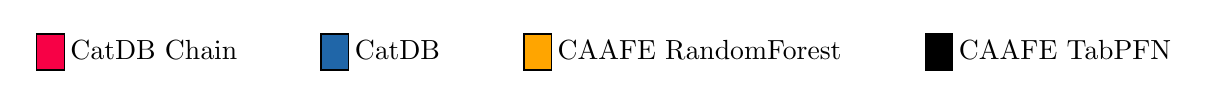
\begin{tikzpicture} 
  \begin{axis}[%
  hide axis,
  xmin=10,
  xmax=50,
  ymin=0,
  ymax=0.4, 
  legend columns=6,
  legend style={draw=white!15!black,legend cell align=left},
  legend style={draw=none, nodes={scale=1, transform shape,}, font=\normalsize},    
  legend image post style={line width=0.5pt,scale=1},
  legend cell align={left},   
  /tikz/every even column/.append style={column sep=2.8em, row sep=0.5em},
  legend image code/.code={\draw [#1] (0cm,-0.23cm) rectangle (0.35cm,0.23cm); }, 
  ]
  \addlegendimage{tug,draw=black, fill=tug,line width=0.3pt}
  \addlegendentry{CatDB Chain};

  \addlegendimage{dblue1,draw=black, fill=dblue1,line width=0.3pt}
  \addlegendentry{CatDB};

  \addlegendimage{color4,draw=black, fill=color4,line width=0.3pt}
  \addlegendentry{CAAFE RandomForest};

  \addlegendimage{black,draw=black, fill=black,line width=0.3pt}
  \addlegendentry{CAAFE TabPFN};
  
  \end{axis}  
\end{tikzpicture}
    %     \caption{Experiment1-Cost-10-Legend}
    % \end{figure}     
    
    % %%%%%%%%%%%%%%%%%%%%%%%%%%%%%%%%%%%%%%%%%%%%%%%%%%%%%%%%%%%%%%%%%%%%%%%%%%%%%%%
    %  \tikzsetnextfilename{Experiment1-Exe-10-Breast-w} 
    %         \begin{figure}[!ht]
    %             \centering
    %             \makeatletter
\newcommand\resetstackedplots{
\makeatletter
\pgfplots@stacked@isfirstplottrue
\makeatother
\addplot [forget plot,draw=none] coordinates{(gemini-1.5-pro-latest, 0) (llama3-70b-8192, 0) (gpt-4o, 0)};
}
\makeatother

\begin{tikzpicture}

  \newcommand{\myaddplotcost}[7]{ 
    \addplot+[xshift=#4,fill=#3, draw=black,line width=0.3pt] 
    table[y=#1, col sep=comma, x=llm_model, discard if singlconfig={No}{#2}{#5}{#6}]
    {../archive/SIGMOD2025-Results/ExeResults.csv};
  };

  \newcommand{\myaddplotds}[6]{
    \resetstackedplots
    \myaddplotcost{CatDB_10_min}{#1}{dblue1}{#3}{#2}{0}{tug};
    \resetstackedplots
    \myaddplotcost{CatDBChain_10_min}{#1}{tug}{#4}{#2}{0}{dred1};    
    \resetstackedplots
    \myaddplotcost{CAAFERandomForest_10_min}{#1}{color4}{#5}{#2}{0}{color4};
    \resetstackedplots
    \myaddplotcost{CAAFETabPFN_10_min}{#1}{black}{#6}{#2}{0}{black};
  };
\pgfplotsset{
    discard if singlconfig/.style n args={4}{
        x filter/.code={
            \edef\tempa{\thisrow{has_description}}
            \edef\tempb{#1}
            \ifx\tempa\tempb
              \edef\tempc{\thisrow{llm_model}}
                \edef\tempd{#2}
                  \ifx\tempc\tempd  
                  %
                      \edef\tempe{\thisrow{dataset_name_orig}}
                      \edef\tempf{#3}
                      \ifx\tempe\tempf
                      %
                        \edef\tempg{\thisrow{samples}}
                        \edef\temph{#4}
                        \ifx\tempg\temph                                      
                        \else
                        \def\pgfmathresult{inf}
                        \fi
                      %      
                      \else
                      \def\pgfmathresult{inf}
                      \fi
                  %                
                  \else
                  \def\pgfmathresult{inf}
                  \fi
            \else
            \def\pgfmathresult{inf}
            \fi			
        }
    },
};   

\begin{axis}[
  ymin=0,
  ybar stacked,
  y tick label style={/pgf/number format/1000 sep={}},
  x tick label style={/pgf/number format/1000 sep={}},  
  scaled y ticks=false,
  axis line style={black, line width=0.3pt},
  enlarge y limits={0.14,upper},
  enlarge x limits=0.07,
  ylabel={Execution Time [min.]},
  xlabel={},
  log ticks with fixed point,
  xtick align=outside,
  xtick pos=left,
  ytick pos=left,
  yticklabel style = {font=\large},
  ylabel style = {font=\large, yshift=0pt, xshift=-5pt},
  height=.53\columnwidth,
  width=.66\columnwidth,
  ymajorgrids=true,
  grid style=dotted,
  minor grid style={gray!70},
  %nodes near coords,
  %every node near coord/.append style={font=\fontsize{0.1pt}{0.1}, rotate=90, xshift=8pt, yshift=0pt},
  every axis plot/.append style={line width=0.4pt,mark options={scale=1.5,solid}},  
  xticklabel style = {font=\normalsize, xshift=0pt, yshift=3pt},
  legend image post style={line width=.5pt},          
  bar width=8pt,         
  ytick={0,10,20,30,40},
  yticklabels={0,10,20,30,40},               
  every x tick/.style={ draw=none},
  xtick = data,
  symbolic x coords={gemini-1.5-pro-latest, llama3-70b-8192, gpt-4o},
  xticklabels={\hspace{0.3cm}Gemini-1.5, \hspace{0.1cm}Llama3-70b, \hspace{-0.64cm}GPT-4o},
  legend image code/.code={\draw [#1] (0cm,-0.1cm) rectangle (0.25cm,0.1cm); }, 
]
 \myaddplotds{gemini-1.5-pro-latest}{Breast-w}{0pt}{8pt}{16pt}{24pt}
 \myaddplotds{llama3-70b-8192}{Breast-w}{-11pt}{-3pt}{5pt}{13pt}
 \myaddplotds{gpt-4o}{Breast-w}{-22pt}{-14pt}{-6pt}{2pt}
\end{axis}

\end{tikzpicture}
    %             \caption{Experiment1-Exe-10-Breast-w}
    %         \end{figure} 
    
    % \tikzsetnextfilename{Experiment1-Exe-10-Credit-g} 
    %         \begin{figure}[!ht]
    %             \centering
    %             \makeatletter
\newcommand\resetstackedplots{
\makeatletter
\pgfplots@stacked@isfirstplottrue
\makeatother
\addplot [forget plot,draw=none] coordinates{(gemini-1.5-pro-latest, 0) (llama3-70b-8192, 0) (gpt-4o, 0)};
}
\makeatother

\begin{tikzpicture}

  \newcommand{\myaddplotcost}[7]{ 
    \addplot+[xshift=#4,fill=#3, draw=black,line width=0.3pt] 
    table[y=#1, col sep=comma, x=llm_model, discard if singlconfig={No}{#2}{#5}{#6}]
    {../archive/SIGMOD2025-Results/ExeResults.csv};
  };

  \newcommand{\myaddplotds}[6]{
    \resetstackedplots
    \myaddplotcost{CatDB_10_min}{#1}{dblue1}{#3}{#2}{0}{tug};
    \resetstackedplots
    \myaddplotcost{CatDBChain_10_min}{#1}{tug}{#4}{#2}{0}{dred1};   
    \resetstackedplots
    \myaddplotcost{CAAFERandomForest_10_min}{#1}{color4}{#5}{#2}{0}{color4};
    \resetstackedplots
    \myaddplotcost{CAAFETabPFN_10_min}{#1}{black}{#6}{#2}{0}{black};
  };
\pgfplotsset{
    discard if singlconfig/.style n args={4}{
        x filter/.code={
            \edef\tempa{\thisrow{has_description}}
            \edef\tempb{#1}
            \ifx\tempa\tempb
              \edef\tempc{\thisrow{llm_model}}
                \edef\tempd{#2}
                  \ifx\tempc\tempd  
                  %
                      \edef\tempe{\thisrow{dataset_name_orig}}
                      \edef\tempf{#3}
                      \ifx\tempe\tempf
                      %
                        \edef\tempg{\thisrow{samples}}
                        \edef\temph{#4}
                        \ifx\tempg\temph                                      
                        \else
                        \def\pgfmathresult{inf}
                        \fi
                      %      
                      \else
                      \def\pgfmathresult{inf}
                      \fi
                  %                
                  \else
                  \def\pgfmathresult{inf}
                  \fi
            \else
            \def\pgfmathresult{inf}
            \fi			
        }
    },
};   

\begin{axis}[
  ymin=0,
  ybar stacked,
  y tick label style={/pgf/number format/1000 sep={}},
  x tick label style={/pgf/number format/1000 sep={}},  
  scaled y ticks=false,
  axis line style={black, line width=0.3pt},
  enlarge y limits={0.14,upper},
  enlarge x limits=0.07,
  ylabel={Execution Time [min.]},
  xlabel={},
  log ticks with fixed point,
  xtick align=outside,
  xtick pos=left,
  ytick pos=left,
  yticklabel style = {font=\large},
  ylabel style = {font=\large, yshift=0pt, xshift=-5pt},
  height=.53\columnwidth,
  width=.66\columnwidth,
  ymajorgrids=true,
  grid style=dotted,
  minor grid style={gray!70},
  %nodes near coords,
  %every node near coord/.append style={font=\fontsize{0.1pt}{0.1}, rotate=90, xshift=8pt, yshift=0pt},
  every axis plot/.append style={line width=0.4pt,mark options={scale=1.5,solid}},  
  xticklabel style = {font=\normalsize, xshift=0pt, yshift=3pt},
  legend image post style={line width=.5pt},          
  bar width=8pt,         
  ytick={0,10,20,30,40,50,60,70,80},
  yticklabels={0,10,20,30,40,50,60,70,80},               
  every x tick/.style={ draw=none},
  xtick = data,
  symbolic x coords={gemini-1.5-pro-latest, llama3-70b-8192, gpt-4o},
  xticklabels={\hspace{0.3cm}Gemini-1.5, \hspace{0.1cm}Llama3-70b, \hspace{-0.64cm}GPT-4o},
  legend image code/.code={\draw [#1] (0cm,-0.1cm) rectangle (0.25cm,0.1cm); }, 
]
 \myaddplotds{gemini-1.5-pro-latest}{Credit-g}{0pt}{8pt}{16pt}{24pt}
 \myaddplotds{llama3-70b-8192}{Credit-g}{-11pt}{-3pt}{5pt}{13pt}
 \myaddplotds{gpt-4o}{Credit-g}{-22pt}{-14pt}{-6pt}{2pt}
\end{axis}

\end{tikzpicture}
    %             \caption{Experiment1-Exe-10-Credit-g}
    %         \end{figure} 

    % \tikzsetnextfilename{Experiment1-Exe-10-Diabetes} 
    %         \begin{figure}[!ht]
    %             \centering
    %             \makeatletter
\newcommand\resetstackedplots{
\makeatletter
\pgfplots@stacked@isfirstplottrue
\makeatother
\addplot [forget plot,draw=none] coordinates{(gemini-1.5-pro-latest, 0) (llama3-70b-8192, 0) (gpt-4o, 0)};
}
\makeatother

\begin{tikzpicture}

  \newcommand{\myaddplotcost}[7]{ 
    \addplot+[xshift=#4,fill=#3, draw=black,line width=0.3pt] 
    table[y=#1, col sep=comma, x=llm_model, discard if singlconfig={No}{#2}{#5}{#6}]
    {../archive/SIGMOD2025-Results/ExeResults.csv};
  };

  \newcommand{\myaddplotds}[6]{
    \resetstackedplots
    \myaddplotcost{CatDBChain_10_min}{#1}{tug}{#3}{#2}{0}{dred1};
    \resetstackedplots
    \myaddplotcost{CatDB_10_min}{#1}{dblue1}{#4}{#2}{0}{tug};
    \resetstackedplots
    \myaddplotcost{CAAFERandomForest_10_min}{#1}{color4}{#5}{#2}{0}{color4};
    \resetstackedplots
    \myaddplotcost{CAAFETabPFN_10_min}{#1}{black}{#6}{#2}{0}{black};
  };
\pgfplotsset{
    discard if singlconfig/.style n args={4}{
        x filter/.code={
            \edef\tempa{\thisrow{has_description}}
            \edef\tempb{#1}
            \ifx\tempa\tempb
              \edef\tempc{\thisrow{llm_model}}
                \edef\tempd{#2}
                  \ifx\tempc\tempd  
                  %
                      \edef\tempe{\thisrow{dataset_name_orig}}
                      \edef\tempf{#3}
                      \ifx\tempe\tempf
                      %
                        \edef\tempg{\thisrow{samples}}
                        \edef\temph{#4}
                        \ifx\tempg\temph                                      
                        \else
                        \def\pgfmathresult{inf}
                        \fi
                      %      
                      \else
                      \def\pgfmathresult{inf}
                      \fi
                  %                
                  \else
                  \def\pgfmathresult{inf}
                  \fi
            \else
            \def\pgfmathresult{inf}
            \fi			
        }
    },
};   

\begin{axis}[
  ymin=0,
  ybar stacked,
  y tick label style={/pgf/number format/1000 sep={}},
  x tick label style={/pgf/number format/1000 sep={}},  
  scaled y ticks=false,
  axis line style={black, line width=0.3pt},
  enlarge y limits={0.14,upper},
  enlarge x limits=0.07,
  ylabel={Execution Time [min.]},
  xlabel={},
  log ticks with fixed point,
  xtick align=outside,
  xtick pos=left,
  ytick pos=left,
  yticklabel style = {font=\large},
  ylabel style = {font=\large, yshift=0pt, xshift=-5pt},
  height=.53\columnwidth,
  width=.66\columnwidth,
  ymajorgrids=true,
  grid style=dotted,
  minor grid style={gray!70},
  %nodes near coords,
  %every node near coord/.append style={font=\fontsize{0.1pt}{0.1}, rotate=90, xshift=8pt, yshift=0pt},
  every axis plot/.append style={line width=0.4pt,mark options={scale=1.5,solid}},  
  xticklabel style = {font=\normalsize, xshift=0pt, yshift=3pt},
  legend image post style={line width=.5pt},          
  bar width=8pt,         
  ytick={0,10,20,30,40,50,60,70,80},
  yticklabels={0,10,20,30,40,50,60,70,80},               
  every x tick/.style={ draw=none},
  xtick = data,
  symbolic x coords={gemini-1.5-pro-latest, llama3-70b-8192, gpt-4o},
  xticklabels={\hspace{0.3cm}Gemini-1.5, \hspace{0.1cm}Llama3-70b, \hspace{-0.64cm}GPT-4o},
  legend image code/.code={\draw [#1] (0cm,-0.1cm) rectangle (0.25cm,0.1cm); }, 
]
 \myaddplotds{gemini-1.5-pro-latest}{Diabetes}{0pt}{8pt}{16pt}{24pt}
 \myaddplotds{llama3-70b-8192}{Diabetes}{-11pt}{-3pt}{5pt}{13pt}
 \myaddplotds{gpt-4o}{Diabetes}{-22pt}{-14pt}{-6pt}{2pt}
\end{axis}

\end{tikzpicture}
    %             \caption{Experiment1-Exe-10-Diabetes}
    %         \end{figure} 

    % \tikzsetnextfilename{Experiment1-Exe-10-Nomao} 
    % \begin{figure}[!ht]
    %     \centering
    %     \makeatletter
\newcommand\resetstackedplots{
\makeatletter
\pgfplots@stacked@isfirstplottrue
\makeatother
\addplot [forget plot,draw=none] coordinates{(gemini-1.5-pro-latest, 0) (llama3-70b-8192, 0) (gpt-4o, 0)};
}
\makeatother

\begin{tikzpicture}

  \newcommand{\myaddplotcost}[7]{ 
    \addplot+[xshift=#4,fill=#3, draw=black,line width=0.3pt] 
    table[y=#1, col sep=comma, x=llm_model, discard if singlconfig={No}{#2}{#5}{#6}]
    {../archive/SIGMOD2025-Results/ExeResults.csv};
  };

  \newcommand{\myaddplotds}[6]{
    \resetstackedplots
    \myaddplotcost{CatDBChain_10_min}{#1}{tug}{#3}{#2}{0}{dred1};
    \resetstackedplots
    \myaddplotcost{CatDB_10_min}{#1}{dblue1}{#4}{#2}{0}{tug};
    \resetstackedplots
    \myaddplotcost{CAAFERandomForest_10_min}{#1}{color4}{#5}{#2}{0}{color4};
    \resetstackedplots
    \myaddplotcost{CAAFETabPFN_10_min}{#1}{black}{#6}{#2}{0}{black};
  };
\pgfplotsset{
    discard if singlconfig/.style n args={4}{
        x filter/.code={
            \edef\tempa{\thisrow{has_description}}
            \edef\tempb{#1}
            \ifx\tempa\tempb
              \edef\tempc{\thisrow{llm_model}}
                \edef\tempd{#2}
                  \ifx\tempc\tempd  
                  %
                      \edef\tempe{\thisrow{dataset_name_orig}}
                      \edef\tempf{#3}
                      \ifx\tempe\tempf
                      %
                        \edef\tempg{\thisrow{samples}}
                        \edef\temph{#4}
                        \ifx\tempg\temph                                      
                        \else
                        \def\pgfmathresult{inf}
                        \fi
                      %      
                      \else
                      \def\pgfmathresult{inf}
                      \fi
                  %                
                  \else
                  \def\pgfmathresult{inf}
                  \fi
            \else
            \def\pgfmathresult{inf}
            \fi			
        }
    },
};   

\begin{axis}[
  ymin=0,
  ybar stacked,
  y tick label style={/pgf/number format/1000 sep={}},
  x tick label style={/pgf/number format/1000 sep={}},  
  scaled y ticks=false,
  axis line style={black, line width=0.3pt},
  enlarge y limits={0.14,upper},
  enlarge x limits=0.07,
  ylabel={Execution Time [min.]},
  xlabel={},
  log ticks with fixed point,
  xtick align=outside,
  xtick pos=left,
  ytick pos=left,
  yticklabel style = {font=\large},
  ylabel style = {font=\large, yshift=0pt, xshift=-5pt},
  height=.53\columnwidth,
  width=.66\columnwidth,
  ymajorgrids=true,
  grid style=dotted,
  minor grid style={gray!70},
  %nodes near coords,
  %every node near coord/.append style={font=\fontsize{0.1pt}{0.1}, rotate=90, xshift=8pt, yshift=0pt},
  every axis plot/.append style={line width=0.4pt,mark options={scale=1.5,solid}},  
  xticklabel style = {font=\normalsize, xshift=0pt, yshift=3pt},
  legend image post style={line width=.5pt},          
  bar width=8pt,         
  ytick={0,15,30,45,60,75,90},
  yticklabels={0,15,30,45,60,75,90},               
  every x tick/.style={ draw=none},
  xtick = data,
  symbolic x coords={gemini-1.5-pro-latest, llama3-70b-8192, gpt-4o},
  xticklabels={\hspace{0.3cm}Gemini-1.5, \hspace{0.1cm}Llama3-70b, \hspace{-0.64cm}GPT-4o},
  legend image code/.code={\draw [#1] (0cm,-0.1cm) rectangle (0.25cm,0.1cm); }, 
]
 \myaddplotds{gemini-1.5-pro-latest}{Nomao}{0pt}{8pt}{16pt}{24pt}
 \myaddplotds{llama3-70b-8192}{Nomao}{-11pt}{-3pt}{5pt}{13pt}
 \myaddplotds{gpt-4o}{Nomao}{-22pt}{-14pt}{-6pt}{2pt}
\end{axis}

\end{tikzpicture}
    %     \caption{Experiment1-Exe-10-Nomao}
    % \end{figure} 

    % \tikzsetnextfilename{Experiment1-Exe-10-Gas-Drift} 
    % \begin{figure}[!ht]
    %     \centering
    %     \makeatletter
\newcommand\resetstackedplots{
\makeatletter
\pgfplots@stacked@isfirstplottrue
\makeatother
\addplot [forget plot,draw=none] coordinates{(gemini-1.5-pro-latest, 0.1) (llama3-70b-8192, 0.1) (gpt-4o, 0.1)};
}
\makeatother

\begin{tikzpicture}

  \newcommand{\myaddplotcost}[7]{ 
    \addplot+[xshift=#4,fill=#3, draw=black,line width=0.3pt] 
    table[y=#1, col sep=comma, x=llm_model, discard if singlconfig={No}{#2}{#5}{#6}]
    {../archive/SIGMOD2025-Results/ExeResults.csv};
  };

  \newcommand{\myaddplotds}[6]{
    \resetstackedplots
    \myaddplotcost{CatDB_10_min}{#1}{dblue1}{#3}{#2}{0}{tug};
    \resetstackedplots
    \myaddplotcost{CatDBChain_10_min}{#1}{tug}{#4}{#2}{0}{dred1};    
    \resetstackedplots
    \myaddplotcost{CAAFERandomForest_10_min}{#1}{color4}{#5}{#2}{0}{color4};
    \resetstackedplots
    \myaddplotcost{CAAFETabPFN_10_min}{#1}{black}{#6}{#2}{0}{black};
  };
\pgfplotsset{
    discard if singlconfig/.style n args={4}{
        x filter/.code={
            \edef\tempa{\thisrow{has_description}}
            \edef\tempb{#1}
            \ifx\tempa\tempb
              \edef\tempc{\thisrow{llm_model}}
                \edef\tempd{#2}
                  \ifx\tempc\tempd  
                  %
                      \edef\tempe{\thisrow{dataset_name_orig}}
                      \edef\tempf{#3}
                      \ifx\tempe\tempf
                      %
                        \edef\tempg{\thisrow{samples}}
                        \edef\temph{#4}
                        \ifx\tempg\temph                                      
                        \else
                        \def\pgfmathresult{inf}
                        \fi
                      %      
                      \else
                      \def\pgfmathresult{inf}
                      \fi
                  %                
                  \else
                  \def\pgfmathresult{inf}
                  \fi
            \else
            \def\pgfmathresult{inf}
            \fi			
        }
    },
};   

\begin{axis}[
  ymin=0.1,
  ybar stacked,
  ymode=log,
  y tick label style={/pgf/number format/1000 sep={}},
  x tick label style={/pgf/number format/1000 sep={}},  
  scaled y ticks=false,
  axis line style={black, line width=0.3pt},
  enlarge y limits={0.14,upper},
  enlarge x limits=0.07,
  ylabel={Execution Time [min.]},
  xlabel={},
  log ticks with fixed point,
  xtick align=outside,
  xtick pos=left,
  ytick pos=left,
  yticklabel style = {font=\large},
  ylabel style = {font=\large, yshift=0pt, xshift=-5pt},
  height=.53\columnwidth,
  width=.66\columnwidth,
  ymajorgrids=true,
  grid style=dotted,
  minor grid style={gray!70},
  %nodes near coords,
  %every node near coord/.append style={font=\fontsize{0.1pt}{0.1}, rotate=90, xshift=8pt, yshift=0pt},
  every axis plot/.append style={line width=0.4pt,mark options={scale=1.5,solid}},  
  xticklabel style = {font=\normalsize, xshift=0pt, yshift=3pt},
  legend image post style={line width=.5pt},          
  bar width=8pt,  
  log origin y=infty,  
  max space between ticks=5,     
  ytick={0.1,1,10,100,1000,10000},
  yticklabels={0,1,10,$10^2$,$10^3$,$10^4$},               
  every x tick/.style={ draw=none},
  xtick = data,
  symbolic x coords={gemini-1.5-pro-latest, llama3-70b-8192, gpt-4o},
  xticklabels={\hspace{0.3cm}Gemini-1.5, \hspace{0.1cm}Llama3-70b, \hspace{-0.64cm}GPT-4o},
  legend image code/.code={\draw [#1] (0cm,-0.1cm) rectangle (0.25cm,0.1cm); }, 
]
 \myaddplotds{gemini-1.5-pro-latest}{Gas-Drift}{0pt}{8pt}{16pt}{24pt}
 \myaddplotds{llama3-70b-8192}{Gas-Drift}{-11pt}{-3pt}{5pt}{13pt}
 \myaddplotds{gpt-4o}{Gas-Drift}{-22pt}{-14pt}{-6pt}{2pt}
\end{axis}

\end{tikzpicture}
    %     \caption{Experiment1-Exe-10-Gas-Drift}
    % \end{figure} 

    % \tikzsetnextfilename{Experiment1-Exe-10-Volkert} 
    % \begin{figure}[!ht]
    %     \centering
    %     \makeatletter
\newcommand\resetstackedplots{
\makeatletter
\pgfplots@stacked@isfirstplottrue
\makeatother
\addplot [forget plot,draw=none] coordinates{(gemini-1.5-pro-latest, 0.1) (llama3-70b-8192, 0.1) (gpt-4o, 0.1)};
}
\makeatother

\begin{tikzpicture}

  \newcommand{\myaddplotcost}[7]{ 
    \addplot+[xshift=#4,fill=#3, draw=black,line width=0.3pt] 
    table[y=#1, col sep=comma, x=llm_model, discard if singlconfig={No}{#2}{#5}{#6}]
    {../archive/SIGMOD2025-Results/ExeResults.csv};
  };

  \newcommand{\myaddplotds}[6]{
    \resetstackedplots
    \myaddplotcost{CatDB_10_min}{#1}{dblue1}{#3}{#2}{0}{tug};
    \resetstackedplots
    \myaddplotcost{CatDBChain_10_min}{#1}{tug}{#4}{#2}{0}{dred1};    
    \resetstackedplots
    \myaddplotcost{CAAFERandomForest_10_min}{#1}{color4}{#5}{#2}{0}{color4};
    \resetstackedplots
    \myaddplotcost{CAAFETabPFN_10_min}{#1}{black}{#6}{#2}{0}{black};
  };
\pgfplotsset{
    discard if singlconfig/.style n args={4}{
        x filter/.code={
            \edef\tempa{\thisrow{has_description}}
            \edef\tempb{#1}
            \ifx\tempa\tempb
              \edef\tempc{\thisrow{llm_model}}
                \edef\tempd{#2}
                  \ifx\tempc\tempd  
                  %
                      \edef\tempe{\thisrow{dataset_name_orig}}
                      \edef\tempf{#3}
                      \ifx\tempe\tempf
                      %
                        \edef\tempg{\thisrow{samples}}
                        \edef\temph{#4}
                        \ifx\tempg\temph                                      
                        \else
                        \def\pgfmathresult{inf}
                        \fi
                      %      
                      \else
                      \def\pgfmathresult{inf}
                      \fi
                  %                
                  \else
                  \def\pgfmathresult{inf}
                  \fi
            \else
            \def\pgfmathresult{inf}
            \fi			
        }
    },
};   

\begin{axis}[
  ymin=0.1,
  ybar stacked,
  ymode=log,
  y tick label style={/pgf/number format/1000 sep={}},
  x tick label style={/pgf/number format/1000 sep={}},  
  scaled y ticks=false,
  axis line style={black, line width=0.3pt},
  enlarge y limits={0.14,upper},
  enlarge x limits=0.07,
  ylabel={Execution Time [min.]},
  xlabel={},
  log ticks with fixed point,
  xtick align=outside,
  xtick pos=left,
  ytick pos=left,
  yticklabel style = {font=\large},
  ylabel style = {font=\large, yshift=0pt, xshift=-5pt},
  height=.53\columnwidth,
  width=.66\columnwidth,
  ymajorgrids=true,
  grid style=dotted,
  minor grid style={gray!70},
  %nodes near coords,
  %every node near coord/.append style={font=\fontsize{0.1pt}{0.1}, rotate=90, xshift=8pt, yshift=0pt},
  every axis plot/.append style={line width=0.4pt,mark options={scale=1.5,solid}},  
  xticklabel style = {font=\normalsize, xshift=0pt, yshift=3pt},
  legend image post style={line width=.5pt},          
  bar width=8pt,  
  log origin y=infty,  
  max space between ticks=5,     
  ytick={0.1,1,10,100,1000},
  yticklabels={0,1,10,$10^2$,$10^3$},               
  every x tick/.style={ draw=none},
  xtick = data,
  symbolic x coords={gemini-1.5-pro-latest, llama3-70b-8192, gpt-4o},
  xticklabels={\hspace{0.3cm}Gemini-1.5, \hspace{0.1cm}Llama3-70b, \hspace{-0.64cm}GPT-4o},
  legend image code/.code={\draw [#1] (0cm,-0.1cm) rectangle (0.25cm,0.1cm); }, 
]
 \myaddplotds{gemini-1.5-pro-latest}{Volkert}{0pt}{8pt}{16pt}{24pt}
 \myaddplotds{llama3-70b-8192}{Volkert}{-11pt}{-3pt}{5pt}{13pt}
 \myaddplotds{gpt-4o}{Volkert}{-22pt}{-14pt}{-6pt}{2pt}
\end{axis}

\end{tikzpicture}
    %     \caption{Experiment1-Exe-10-Volkert}
    % \end{figure}             

    % \tikzsetnextfilename{Experiment1-Exe-10-Legend} 
    % \begin{figure}[!ht]
    %     \centering
    %     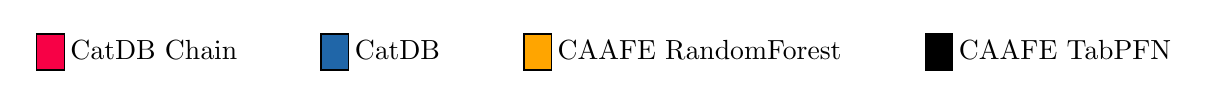
\begin{tikzpicture} 
  \begin{axis}[%
  hide axis,
  xmin=10,
  xmax=50,
  ymin=0,
  ymax=0.4, 
  legend columns=6,
  legend style={draw=white!15!black,legend cell align=left},
  legend style={draw=none, nodes={scale=1, transform shape,}, font=\normalsize},    
  legend image post style={line width=0.5pt,scale=1},
  legend cell align={left},   
  /tikz/every even column/.append style={column sep=2.8em, row sep=0.5em},
  legend image code/.code={\draw [#1] (0cm,-0.23cm) rectangle (0.35cm,0.23cm); }, 
  ]
  \addlegendimage{tug,draw=black, fill=tug,line width=0.3pt}
  \addlegendentry{CatDB Chain};

  \addlegendimage{dblue1,draw=black, fill=dblue1,line width=0.3pt}
  \addlegendentry{CatDB};

  \addlegendimage{color4,draw=black, fill=color4,line width=0.3pt}
  \addlegendentry{CAAFE RandomForest};

  \addlegendimage{black,draw=black, fill=black,line width=0.3pt}
  \addlegendentry{CAAFE TabPFN};
  
  \end{axis}  
\end{tikzpicture}
    %     \caption{Experiment1-Exe-10-Legend}
    % \end{figure}    
            
      

    %  \tikzsetnextfilename{Experiment1-Cost-Legend} 
    %     \begin{figure}[!ht]
    %         \centering
    %         \begin{tikzpicture} 
  \begin{axis}[%
  hide axis,
  xmin=10,
  xmax=50,
  ymin=0,
  ymax=0.4, 
  legend columns=6,
  legend style={draw=white!15!black,legend cell align=left},
  legend style={draw=none, nodes={scale=1, transform shape,}, font=\huge},    
  legend image post style={line width=0.5pt,scale=1},
  legend cell align={left},   
  /tikz/every even column/.append style={column sep=2.8em, row sep=0.5em},
  legend image code/.code={\draw [#1] (0cm,-0.23cm) rectangle (0.35cm,0.23cm); }, 
  ]
  \addlegendimage{dblue1,draw=black, fill=dblue1,line width=0.3pt}
  \addlegendentry{CatDB Chain};

  \addlegendimage{dred1,draw=black, fill=dred1,line width=0.3pt}
  \addlegendentry{CatDB Chain Error};

  \addlegendimage{dblue2,draw=black, fill=dblue2,line width=0.3pt}
  \addlegendentry{CatDB Chain PP$^{*}$};

  \addlegendimage{dred2,draw=black, fill=dred2,line width=0.3pt}
  \addlegendentry{CatDB Chain PP$^{*}$ Error};

  \addlegendimage{dblue3,draw=black, fill=dblue3,line width=0.3pt}
  \addlegendentry{CatDB Chain FE$^{*}$};

  \addlegendimage{dred3,draw=black, fill=dred3,line width=0.3pt}
  \addlegendentry{CatDB FE$^{*}$ Error};

  \addlegendimage{dblue1,draw=black, fill=color6,line width=0.3pt}
  \addlegendentry{CatDB};

  \addlegendimage{dblue1,draw=black, fill=tug,line width=0.3pt}
  \addlegendentry{CatDB Error};

  \addlegendimage{color4,draw=black, fill=color4,line width=0.3pt}
  \addlegendentry{CAAFE RandomForest};

  \addlegendimage{black,draw=black, fill=black,line width=0.3pt}
  \addlegendentry{CAAFE TabPFN};
  
  \end{axis}
  \node[draw=gray, fill=lightgray!30,font=\huge, xshift=0pt] at (rel axis cs: 0.18,0.79){PP$^{*}$ = Pre-processing  \ \ \ \ \ FE $^{*}$ = Feature Engineering};  
\end{tikzpicture}
    %         \caption{Experiment1-Cost-Legend}
    %     \end{figure}    

    %   \tikzsetnextfilename{Experiment1-OverAll-Gemini} 
    %     \begin{figure}[!ht]
    %         \centering
    %         \makeatletter
\newcommand\resetstackedplots{
\makeatletter
\pgfplots@stacked@isfirstplottrue
\makeatother
\addplot [forget plot,draw=none] coordinates{(Skin,0) (Diabetes,0) (Tic-Tac-Toe,0) (Breast-w,0) (Credit-g,0 )(Higgs,0) (Nomao,0) (Balance-Scale,0) (Walking-Activity,0) (Jungle-Chess,0) (CMC,0) (Traffic,0) (Gas-Drift,0) (Volkert,0) (Black-Friday,0) (Bike-Sharing,0)(NYC,0) (House-Sales,0)};
}
\makeatother

\begin{tikzpicture}
    \newcommand{\addplotOverAll}[4]{        
        \addplot[xshift=#4,fill=#3,draw=black,discard if single={#1}, line width=0.2pt]
        table[ y=#2, col sep=comma, x=dataset_name] {../archive/SIGMOD2025-Results/OverallResults.csv};
        \label{#2}
    };   
   
    \newcommand{\myaddplotllm}[1]{
      \resetstackedplots
      \addplotOverAll{#1}{CatDB}{tugb}{-3.5pt};
      \resetstackedplots
      \addplotOverAll{#1}{CatDBChain}{tug}{0pt};
      \resetstackedplots
      \addplotOverAll{#1}{max_other}{black}{3.5pt};      
    };

    \pgfplotsset{
        discard if single/.style n args={1}{
            x filter/.code={
                \edef\tempa{\thisrow{llm_model}}
                \edef\tempb{#1}
                \ifx\tempa\tempb
                \else
                \def\pgfmathresult{inf}
                \fi
            }
        }
    };
   

\begin{axis}[
  ybar stacked,
  ymin=0,
  ymax=100,
  y tick label style={/pgf/number format/1000 sep={}},
  x tick label style={/pgf/number format/1000 sep={}},  
  scaled y ticks=false,
  axis line style={black, line width=0.3pt},
  enlarge y limits={0.35,upper},
  enlarge x limits=0.03,
  ylabel={AUC/AUC-over/$R^2$ [\%]},
  xlabel={$\#$ Dataset},
  log ticks with fixed point,
  xtick align=outside,
  xtick pos=left,
  ytick pos=left,
  yticklabel style = {font=\normalsize},
  ylabel style = {font=\normalsize, yshift=-6pt, xshift=-4pt},
  height=.5\columnwidth,
  width=1.3\columnwidth,
  ymajorgrids=true,
  grid style=dotted,
  minor grid style={gray!70},
  every axis plot/.append style={line width=0.4pt,mark options={scale=1.5,solid}},  
  xticklabel style = {font=\normalsize, xshift=0pt, yshift=4pt},
  legend image post style={line width=.5pt},          
  bar width=3.5pt,         
  % ytick={0,20,40,60,80,100},
  % yticklabels={0, 20, 40, 60, 80, 100},               
  every x tick/.style={ draw=none},
  xtick = data,
  symbolic x coords={Skin,Diabetes,Tic-Tac-Toe,Breast-w,Credit-g,Higgs,Nomao,Balance-Scale,Walking-Activity,Jungle-Chess,CMC,Traffic,Gas-Drift,Volkert,Black-Friday,Bike-Sharing,NYC,House-Sales},
  xticklabels={1,2,3,4,5,6,7,8,9,10,11,12,13,14,15,16,17,18},
  legend image code/.code={\draw [#1] (0cm,-0.1cm) rectangle (0.15cm,0.1cm); }, 
]
\myaddplotllm{gemini-1.5-pro-latest}
\end{axis}

\node [draw=none,inner sep=0, font=\footnotesize, anchor=west] (leg1) at (rel axis cs: 0.06,0.9) {\shortstack[l]{
  \ref{CatDB} CatDB \ \ \ref{CatDBChain} CatDB Chain \ \ \ref{max_other} Maximum Performance of Baselines (CAAFE \& AutoML)
  }};

\end{tikzpicture}

    %         \caption{Experiment1-OverAll-Gemini}
    %     \end{figure}   
        
    %     \tikzsetnextfilename{Experiment1-OverAll-LLama} 
    %     \begin{figure}[!ht]
    %         \centering
    %         \makeatletter
\newcommand\resetstackedplots{
\makeatletter
\pgfplots@stacked@isfirstplottrue
\makeatother
\addplot [forget plot,draw=none] coordinates{(Balance-Scale, 0) (Breast-w, 0) (CMC, 0) (Credit-g, 0) (Diabetes, 0) (Tic-Tac-Toe, 0) (Eucalyptus, 0) (PC1, 0) (Jungle-Chess, 0) (Higgs, 0) (Skin, 0) (Traffic, 0) (Walking-Activity, 0) (Black-Friday, 0) (Bike-Sharing, 0) (House-Sales, 0) (NYC, 0) (Airlines-DepDelay,0)};
}
\makeatother

\begin{tikzpicture}
    \newcommand{\addplotOverAll}[4]{        
        \addplot[xshift=#4,fill=#3,draw=black,discard if single={#1}, line width=0.3pt]
        table[ y=#2, col sep=comma, x=dataset_name] {../archive/SIGMOD2025-Results/OverallResults.csv};
        \label{#2}
    };   
   
    \newcommand{\myaddplotllm}[1]{
      \resetstackedplots
      \addplotOverAll{#1}{CatDB}{tugb}{-3.5pt};
      \resetstackedplots
      \addplotOverAll{#1}{CatDBChain}{tug}{0pt};
      \resetstackedplots
      \addplotOverAll{#1}{max_other}{black}{3.5pt};      
    };

    \pgfplotsset{
        discard if single/.style n args={1}{
            x filter/.code={
                \edef\tempa{\thisrow{llm_model}}
                \edef\tempb{#1}
                \ifx\tempa\tempb
                \else
                \def\pgfmathresult{inf}
                \fi
            }
        }
    };
   

\begin{axis}[
  ybar stacked,
  ymin=0,
  ymax=100,
  y tick label style={/pgf/number format/1000 sep={}},
  x tick label style={/pgf/number format/1000 sep={}},  
  scaled y ticks=false,
  axis line style={black, line width=0.3pt},
  enlarge y limits={0.35,upper},
  enlarge x limits=0.03,
  ylabel={AUC/AUC-over/$R^2$ [\%]},
  xlabel={$\#$ Dataset},
  log ticks with fixed point,
  xtick align=outside,
  xtick pos=left,
  ytick pos=left,
  yticklabel style = {font=\normalsize},
  ylabel style = {font=\normalsize, yshift=-6pt, xshift=-4pt},
  height=.5\columnwidth,
  width=1.3\columnwidth,
  ymajorgrids=true,
  grid style=dotted,
  minor grid style={gray!70},
  every axis plot/.append style={line width=0.4pt,mark options={scale=1.5,solid}},  
  xticklabel style = {font=\normalsize, xshift=0pt, yshift=4pt},
  legend image post style={line width=.5pt},          
  bar width=3.5pt,         
  ytick={0,20,40,60,80,100},
  yticklabels={0, 20, 40, 60, 80, 100},               
  every x tick/.style={ draw=none},
  xtick = data,
  symbolic x coords={Balance-Scale,Breast-w,CMC,Credit-g,Diabetes,Tic-Tac-Toe,Eucalyptus,PC1,Jungle-Chess,Higgs,Skin,Traffic,Walking-Activity,Black-Friday,Bike-Sharing,House-Sales,NYC,Airlines-DepDelay},
  xticklabels={1,2,3,4,5,6,7,8,9,10,11,12,13,14,15,16,17,18},
  legend image code/.code={\draw [#1] (0cm,-0.1cm) rectangle (0.15cm,0.1cm); }, 
]
\myaddplotllm{llama3-70b-8192}

\end{axis}

\node [draw=none,inner sep=0, font=\footnotesize, anchor=west] (leg1) at (rel axis cs: 0.06,0.9) {\shortstack[l]{
  \ref{CatDB} CatDB \ \ \ref{CatDBChain} CatDB Chain \ \ \ref{max_other} Maximum Performance of Baselines (CAAFE \& AutoML)
  }};

\end{tikzpicture}

    %         \caption{Experiment1-OverAll-LLama}
    %     \end{figure}   
        
    %     \tikzsetnextfilename{Experiment1-OverAll-GPT} 
    %     \begin{figure}[!ht]
    %         \centering
    %         \makeatletter
\newcommand\resetstackedplots{
\makeatletter
\pgfplots@stacked@isfirstplottrue
\makeatother
\addplot [forget plot,draw=none] coordinates{(Balance-Scale, 0) (Breast-w, 0) (CMC, 0) (Credit-g, 0) (Diabetes, 0) (Tic-Tac-Toe, 0) (Eucalyptus, 0) (PC1, 0) (Jungle-Chess, 0) (Higgs, 0) (Skin, 0) (Traffic, 0) (Walking-Activity, 0) (Black-Friday, 0) (Bike-Sharing, 0) (House-Sales, 0) (NYC, 0) (Airlines-DepDelay,0)};
}
\makeatother

\begin{tikzpicture}
    \newcommand{\addplotOverAll}[4]{        
        \addplot[xshift=#4,fill=#3,draw=black,discard if single={#1}, line width=0.3pt]
        table[ y=#2, col sep=comma, x=dataset_name] {../archive/SIGMOD2025-Results/OverallResults.csv};
        \label{#2}
    };   
   
    \newcommand{\myaddplotllm}[1]{
      \resetstackedplots
      \addplotOverAll{#1}{CatDB}{tugb}{-3.5pt};
      \resetstackedplots
      \addplotOverAll{#1}{CatDBChain}{tug}{0pt};
      \resetstackedplots
      \addplotOverAll{#1}{max_other}{black}{3.5pt};      
    };

    \pgfplotsset{
        discard if single/.style n args={1}{
            x filter/.code={
                \edef\tempa{\thisrow{llm_model}}
                \edef\tempb{#1}
                \ifx\tempa\tempb
                \else
                \def\pgfmathresult{inf}
                \fi
            }
        }
    };
   

\begin{axis}[
  ybar stacked,
  ymin=0,
  ymax=100,
  y tick label style={/pgf/number format/1000 sep={}},
  x tick label style={/pgf/number format/1000 sep={}},  
  scaled y ticks=false,
  axis line style={black, line width=0.3pt},
  enlarge y limits={0.35,upper},
  enlarge x limits=0.03,
  ylabel={AUC/AUC-over/$R^2$ [\%]},
  xlabel={$\#$ Dataset},
  log ticks with fixed point,
  xtick align=outside,
  xtick pos=left,
  ytick pos=left,
  yticklabel style = {font=\normalsize},
  ylabel style = {font=\normalsize, yshift=-6pt, xshift=-4pt},
  height=.5\columnwidth,
  width=1.3\columnwidth,
  ymajorgrids=true,
  grid style=dotted,
  minor grid style={gray!70},
  every axis plot/.append style={line width=0.4pt,mark options={scale=1.5,solid}},  
  xticklabel style = {font=\normalsize, xshift=0pt, yshift=4pt},
  legend image post style={line width=.5pt},          
  bar width=3.5pt,         
  ytick={0,20,40,60,80,100},
  yticklabels={0, 20, 40, 60, 80, 100},               
  every x tick/.style={ draw=none},
  xtick = data,
  symbolic x coords={Balance-Scale,Breast-w,CMC,Credit-g,Diabetes,Tic-Tac-Toe,Eucalyptus,PC1,Jungle-Chess,Higgs,Skin,Traffic,Walking-Activity,Black-Friday,Bike-Sharing,House-Sales,NYC,Airlines-DepDelay},
  xticklabels={1,2,3,4,5,6,7,8,9,10,11,12,13,14,15,16,17,18},
  legend image code/.code={\draw [#1] (0cm,-0.1cm) rectangle (0.15cm,0.1cm); }, 
]
\myaddplotllm{gpt-4o}

\end{axis}

\node [draw=none,inner sep=0, font=\footnotesize, anchor=west] (leg1) at (rel axis cs: 0.06,0.9) {\shortstack[l]{
  \ref{CatDB} CatDB \ \ \ref{CatDBChain} CatDB Chain \ \ \ref{max_other} Maximum Performance of Baselines (CAAFE \& AutoML)
  }};

\end{tikzpicture}

    %         \caption{Experiment1-OverAll-GPT}
    %     \end{figure}   
    
\end{document}
\endinput
